%%%%%%%%%%%%%%%%%%%%%%%%%%%%%%%%%%%%%%%%%
% kaobook
% LaTeX Template
% Version 1.3 (December 9, 2021)
%
% This template originates from:
% https://www.LaTeXTemplates.com
%
% For the latest template development version and to make contributions:
% https://github.com/fmarotta/kaobook
%
% Authors:
% Federico Marotta (federicomarotta@mail.com)
% Based on the doctoral thesis of Ken Arroyo Ohori (https://3d.bk.tudelft.nl/ken/en)
% and on the Tufte-LaTeX class.
% Modified for LaTeX Templates by Vel (vel@latextemplates.com)
%
% License:
% CC0 1.0 Universal (see included MANIFEST.md file)
%
%%%%%%%%%%%%%%%%%%%%%%%%%%%%%%%%%%%%%%%%%

%----------------------------------------------------------------------------------------
%	PACKAGES AND OTHER DOCUMENT CONFIGURATIONS
%----------------------------------------------------------------------------------------

\documentclass[
a4paper, % Page size
fontsize=10pt, % Base font size
twoside=true, % Use different layouts for even and odd pages (in particular, if twoside=true, the margin column will be always on the outside)
%open=any, % If twoside=true, uncomment this to force new chapters to start on any page, not only on right (odd) pages
%chapterentrydots=true, % Uncomment to output dots from the chapter name to the page number in the table of contents
numbers=noenddot, % Comment to output dots after chapter numbers; the most common values for this option are: enddot, noenddot and auto (see the KOMAScript documentation for an in-depth explanation)
]{kaobook}

% Choose the language
\ifxetexorluatex
\usepackage{polyglossia}
\setmainlanguage{spanish}
\setotherlanguage{english}
\else
\usepackage[spanish, mexico-com]{babel} % Load characters and hyphenation
\fi
\usepackage[spanish=mexican]{csquotes}	% Spanish quotes

% Load packages for testing
\usepackage{blindtext}
%\usepackage{showframe} % Uncomment to show boxes around the text area, margin, header and footer
%\usepackage{showlabels} % Uncomment to output the content of \label commands to the document where they are used

%-------------------------------------------------------------
%   MY ADDS
%-------------------------------------------------------------
%\usepackage{adjmulticol}
\usepackage{tikz}
\usetikzlibrary{calc, patterns}
\usepackage{tikz-dimline}
\usepackage{pgfplots}  % Gráfica de funciones

\usepackage{amssymb, amsfonts, mathtools, bm}  % Matemática. kaobook ya carga amsmath
\usepackage{siunitx}  % Unidades del SI.
\usepackage{blkarray}  % Para indicar filas y columnas en matrices
\usepackage{subcaption}  % Caption a subfiguras
\usepackage[most]{tcolorbox}  % Cuadros de colores
\usepackage{standalone}  % para generar gráficos en archivos separados
\usepackage{systeme}  % Para escribir sistemas de ecuaciones
\usepackage{cancel}  % Para tachar términos en ecuaciones
\usepackage{nomencl}  % Para crear nomenclatura
\makenomenclature

% Mis colores
\definecolor{tt1}{RGB}{210, 214, 217}
\definecolor{tt2}{RGB}{186, 189, 191}
\definecolor{tt3}{RGB}{240, 241, 242}
\definecolor{tt4}{RGB}{115, 114, 114}
\definecolor{tt5}{RGB}{38, 26, 23}
%


%Para repetir figuras con la misma enumeración
\newcommand{\repeatcaption}[2]{%
	\renewcommand{\thefigure}{\ref{#1}}%
	\captionsetup{list=no}%
	\caption{#2 (repetido de la pág. \pageref{#1}).}%
	\addtocounter{figure}{-1}% So that next figure after the repeat gets the right number.
}

%---------------------------
% THE END OF MY ADDS
%---------------------------


% Load the bibliography package
\usepackage{kaobiblio}
\addbibresource{./bibs/bef.bib} % Bibliography file

% Load mathematical packages for theorems and related environments
\usepackage[framed=true]{kaotheorems}

% Load the package for hyperreferences
\usepackage{kaorefs}

\graphicspath{{figs/}, {images/}} % Paths in which to look for images

\makeindex[columns=3, title=Alphabetical Index, intoc] % Make LaTeX produce the files required to compile the index

\makeglossaries % Make LaTeX produce the files required to compile the glossary
\newacronym{cfe}{CFE}{Condiciones de frontera esenciales}
\newacronym{cfn}{CFN}{Condiciones de frontera naturales} % Include the glossary definitions

\makenomenclature % Make LaTeX produce the files required to compile the nomenclature

% Reset sidenote counter at chapters
%\counterwithin*{sidenote}{chapter}

%----------------------------------------------------------------------------------------

\begin{document}
	% Mis macros
	\newcommand{\Titulo}{Introducción a elementos finitos}
\newcommand{\subTitulo}{con algoritmos en python}
\newcommand{\yo}{Fredy Gabriel Ramírez Villanueva}
\newcommand{\fecha}{\today}
	
	\frontmatter % Parte introductoria
	
	% Portada
	%!TEX root = ../main.tex
\newgeometry{left=4cm}

\begin{titlepage}
	\begin{center}
	
		\includegraphics[width=.2\textwidth]{figs/portada/LogoFCyT}
		
		\Large
		\textbf{Universidad Nacional de Caaguazú}
		
		\vspace{0.3cm}
		\Large
		Facultad de Ciencias y Tecnologías
		
		\vspace{1.2cm}
		
		\textbf{\Titulo}
		
		\subTitulo
		
		\vspace{1cm}
		
		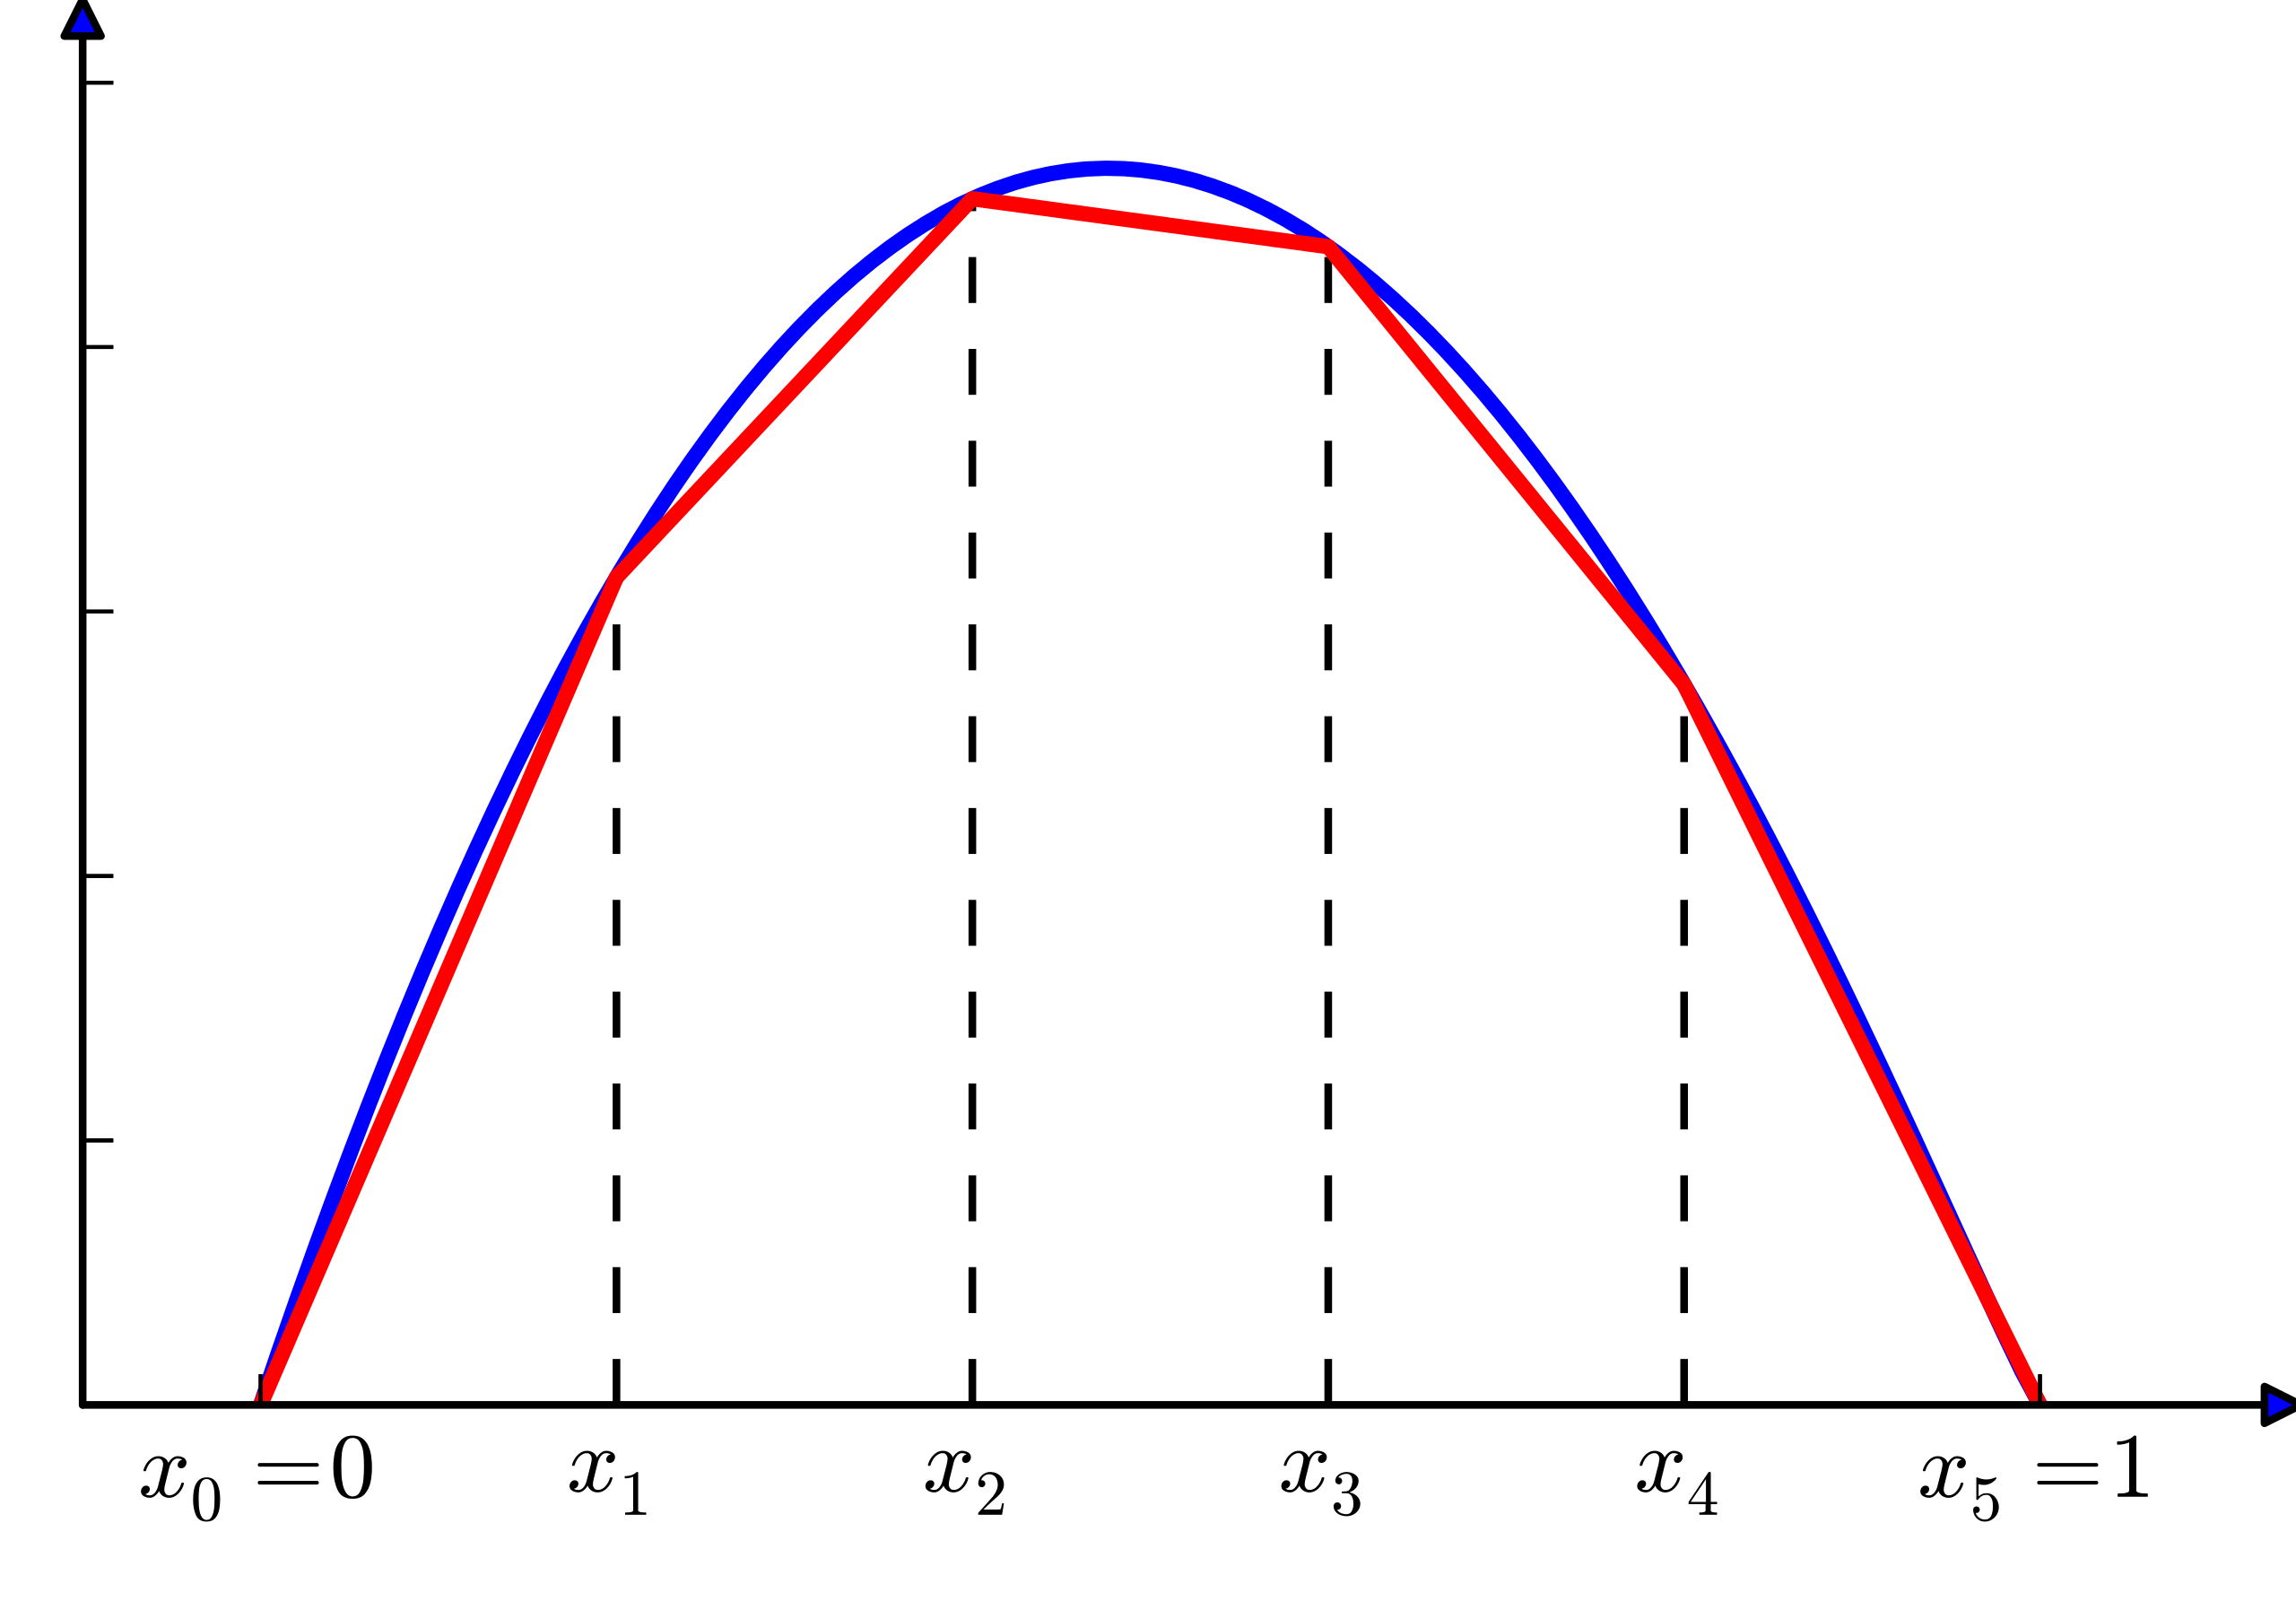
\includegraphics[width=0.4\textwidth]{figs/portada/fem}
		
		\vspace{1cm}
		
		\textbf{\yo}
		
		Ing. Civil, M.Sc.
		
		\vspace{0.8cm}
		
		\large
		Coronel Oviedo - Paraguay
		
		\fecha
		\vspace{.5cm}
		
		Material en elaboración: versión 0.1.0-alpha
	\end{center}
\end{titlepage}

\restoregeometry
	% \cleardoublepage
	
	\tableofcontents
	\listoffigures
	\listoftables
	\printnomenclature[1.2cm]
	
	\mainmatter %Parte principal
	
	% Capítulos
	%	%!TEX root = ../main.tex

\setchapterimage[7.5cm]{figs/intro/highway}
\setchapterpreamble[u]{\margintoc}


\chapter{Introducción} \label{chap:intro}

\begin{kaobox}
	``Los científicos investigan lo que ya es; los ingenieros crean lo que nunca ha sido”
\begin{flushright}
	Albert Einstein
\end{flushright}
\end{kaobox}


\section{Lista de ideas}

\begin{enumerate}
	\item El libro debe tener su página web
	\item Me gustaría que gran parte sea open source, por ejemplo los códigos de python, podría ser también los Tikz de las figuras y otros deberían estar disponible para todos en GitHub. Pero el formato impreso (o digital completo) y los videos me gustaría monetizar;
	\item Cada ejercicio o alguna parte importante, puede tener un video asociado, y puesto en el libro como QR el enlace del video.
	\item Como imagen del capítulo se podría utilizar fotos de estructuras importantes del Paraguay.
	\item Cada capítulo pordría empezar con una frase inspiradora de ingenieros famosos, seguida de un resumen del capítulo.
	\item Usar cuadros de recordatorios a los márgenes para recordar algún concepto o parar repetir brevemento lo ya dicho en una sección anterior.
	\item El punto central es facilitar al máximo la lectura y el acceso de los recursos del libro.
\end{enumerate}


\section{En este capítulo}

\begin{enumerate}
	\item Introducción a los elementos finitos
	\item Notas históricas
	\item Aplicaciones
\end{enumerate}

\section{En este o en otro capítulo}

\begin{itemize}
	\item Base matemática
	\item Ecuaciones diferenciales y condiciones de frontera
	\item Álgebra lineal
	\item Cálculo variacional
\end{itemize}

El análisis estructural es una disciplina fundamental en la ingeniería civil, mecánica y aeroespacial, entre otras.  Su objetivo principal es determinar el comportamiento de estructuras bajo diversas condiciones de carga, lo que permite predecir su resistencia, rigidez y estabilidad.  Tradicionalmente, el análisis estructural se ha basado en métodos analíticos para resolver las ecuaciones que gobiernan el comportamiento de las estructuras. Sin embargo, estos métodos tienen limitaciones cuando se trata de analizar estructuras complejas con geometrías irregulares, materiales no lineales o condiciones de carga complejas.

Es aquí donde el Método de los Elementos Finitos (MEF) emerge como una herramienta poderosa y versátil. El MEF es una técnica numérica que permite aproximar la solución de ecuaciones diferenciales que describen fenómenos físicos, como el comportamiento de estructuras bajo cargas.  A diferencia de los métodos analíticos, el MEF puede manejar geometrías complejas, materiales no lineales y condiciones de carga arbitrarias, lo que lo convierte en una herramienta indispensable para el análisis de estructuras modernas.

%\begin{figure}[h]
%	\centering
%	\includegraphics[width=0.8\textwidth]{ejemplo_mef_puente.jpg} % Reemplaza con una imagen de un puente analizado con MEF
%	\caption{Ejemplo de análisis de un puente mediante el Método de los Elementos Finitos.  (Imagen de referencia, reemplazar por una imagen real)}
%\end{figure}

El MEF se basa en la discretización del dominio de la estructura en un conjunto de elementos finitos interconectados.  Cada elemento se representa mediante un conjunto de ecuaciones algebraicas que aproximan el comportamiento del elemento. Al ensamblar las ecuaciones de todos los elementos, se obtiene un sistema global de ecuaciones que describe el comportamiento de la estructura completa.  La solución de este sistema de ecuaciones proporciona información sobre los desplazamientos, deformaciones y esfuerzos en la estructura.

En este libro, exploraremos los fundamentos del MEF y su aplicación al análisis estructural.  Abordaremos los siguientes temas:

\textbf{Bases matemáticas:} Repasaremos los conceptos matemáticos necesarios para comprender el MEF, incluyendo álgebra lineal, cálculo diferencial e integral, y ecuaciones diferenciales.

\textbf{Conceptos fundamentales del MEF:}  Estudiaremos los principios básicos del MEF, como la discretización del dominio, las funciones de forma, el ensamblaje de matrices y la aplicación de condiciones de contorno.

\textbf{Métodos aproximados:}  Analizaremos métodos aproximados como el método de Rayleigh-Ritz y el método de Galerkin, que son la base del MEF.

\textbf{Elementos finitos de 1, 2 y 3 dimensiones:}  Derivamos las ecuaciones de elementos finitos para diferentes tipos de elementos, incluyendo barras, vigas, placas y sólidos.

\textbf{Aplicaciones:} Resolveremos problemas de análisis estructural utilizando el MEF, incluyendo ejemplos de estructuras de barras, vigas y marcos, placas y láminas, y sólidos tridimensionales.
	
Además, a lo largo del libro utilizaremos el lenguaje de programación Python para implementar los conceptos del MEF y resolver problemas de análisis estructural.  Python es un lenguaje versátil y popular en la comunidad científica e ingenieril, con una amplia gama de bibliotecas para el cálculo numérico, la visualización y el análisis de datos.  Al combinar la teoría del MEF con la práctica en Python, este libro te proporcionará las herramientas necesarias para comprender y aplicar el MEF en problemas reales de ingeniería.
	%!TEX root = ../main.tex
\setchapterimage[7.5cm]{figs/mate-bases/rotonda_czu1}
\setchapterpreamble[u]{\margintoc}

\chapter{Bases matemáticas} \label{chap:mate}

\begin{kaobox}
	``La naturaleza está escrita en lenguaje matemático"
	\begin{flushright}
		Galileo Galilei
	\end{flushright}
\end{kaobox}

Breve resumen histórico, basado en \cite{GoodVibrations01}

Alrededor del año 1670 el Cálculo fue inventado por Newton y/o Leibniz quienes tuvieron
la conocida controversia por los créditos de la creación de tan importante rama de la
matemática \cite{guicciardini2003reading}.

En 1687 fue publicado Philosophiæ naturalis principia mathematica (en latín) de Sir Isaac Newton \cite{newton1987}.

1696 Johann Bernoulli, problema de la braquistócrona.

1733 Euler abordó el problema de la braquistócrona.

1743 Principio de D'Alembert

1755 Lagrange a los 19 años, problema de la tautócrona.

1756 Euler, cálculo de variaciones.

1788 Lagrange, Mecánica Analítica

1834 Principio de Hamilton


\section{Álgebra lineal}
\subsection{Operaciones con matrices}

Inspirado en el enfoque claro y conciso del libro ``Linear Algebra and Its Applications'' de Gilbert Strang, este capítulo introduce el concepto fundamental de las matrices y las operaciones básicas que se pueden realizar con ellas. Las matrices son arreglos rectangulares de números que desempeñan un papel esencial en diversas áreas de las matemáticas, la física, la ingeniería y la computación.  Su capacidad para representar y manipular datos de forma eficiente las convierte en una herramienta indispensable en el análisis de sistemas lineales y en la resolución de problemas complejos.

\subsubsection{¿Qué es una Matriz?}

Una matriz es un arreglo rectangular de números, símbolos o expresiones, organizados en filas y columnas.  Cada número dentro de la matriz se denomina elemento o entrada.  

\begin{equation*}
	A = \begin{bmatrix}
		a_{11} & a_{12} & \cdots & a_{1n} \\
		a_{21} & a_{22} & \cdots & a_{2n} \\
		\vdots & \vdots & \ddots & \vdots \\
		a_{m1} & a_{m2} & \cdots & a_{mn} 
	\end{bmatrix}
\end{equation*}

En esta matriz $A$, $a_{ij}$ representa el elemento ubicado en la fila $i$ y la columna $j$.  El tamaño de una matriz se define por su número de filas ($m$) y su número de columnas ($n$), y se denota como $m \times n$.  Por ejemplo, la matriz $A$ mostrada arriba es una matriz $m \times n$.

\subsubsection{Operaciones con Matrices}

\begin{itemize}
	\item Suma y Resta de Matrices
	
	La suma y la resta de matrices se definen solo para matrices del mismo tamaño.  Para sumar o restar dos matrices, simplemente se suman o restan los elementos correspondientes.
	
	Si $A = [a_{ij}]$ y $B = [b_{ij}]$ son dos matrices $m \times n$, entonces su suma $C = A + B$ es una matriz $m \times n$ donde $c_{ij} = a_{ij} + b_{ij}$.
	
	\begin{example}
		Si $A = \begin{bmatrix} 1 & 2 \\ 3 & 4 \end{bmatrix}$ y $B = \begin{bmatrix} 5 & 6 \\ 7 & 8 \end{bmatrix}$, entonces 
		$A + B = \begin{bmatrix} 1+5 & 2+6 \\ 3+7 & 4+8 \end{bmatrix} = \begin{bmatrix} 6 & 8 \\ 10 & 12 \end{bmatrix}$.
	\end{example}
	
	\item Multiplicación por un Escalar
	
	Para multiplicar una matriz por un escalar, se multiplica cada elemento de la matriz por ese escalar.
	
	Si $A = [a_{ij}]$ es una matriz $m \times n$ y $k$ es un escalar, entonces el producto $kA$ es una matriz $m \times n$ donde cada elemento es $ka_{ij}$.
	
	\begin{example}
		Si $A = \begin{bmatrix} 1 & 2 \\ 3 & 4 \end{bmatrix}$ y $k = 3$, entonces 
		$kA = \begin{bmatrix} 3 \cdot 1 & 3 \cdot 2 \\ 3 \cdot 3 & 3 \cdot 4 \end{bmatrix} = \begin{bmatrix} 3 & 6 \\ 9 & 12 \end{bmatrix}$.
	\end{example}
	
	\item Multiplicación de Matrices
	
	La multiplicación de matrices es una operación más compleja que la suma y la resta.  Dos matrices $A$ y $B$ pueden multiplicarse solo si el número de columnas de $A$ es igual al número de filas de $B$.
	
	Si $A = [a_{ij}]$ es una matriz $m \times n$ y $B = [b_{ij}]$ es una matriz $n \times p$, entonces su producto $C = AB$ es una matriz $m \times p$ donde el elemento $c_{ij}$ se calcula como:
	
	\begin{equation*}
		c_{ij} = a_{i1}b_{1j} + a_{i2}b_{2j} + \cdots + a_{in}b_{nj} 
	\end{equation*}
	
	En otras palabras, para obtener el elemento $c_{ij}$, se multiplican los elementos de la fila $i$ de $A$ por los elementos correspondientes de la columna $j$ de $B$, y se suman los productos.
	
	\begin{example}
		Si $A = \begin{bmatrix} 1 & 2 \\ 3 & 4 \end{bmatrix}$ y $B = \begin{bmatrix} 5 & 6 \\ 7 & 8 \end{bmatrix}$, entonces 
		$AB = \begin{bmatrix} 1 \cdot 5 + 2 \cdot 7 & 1 \cdot 6 + 2 \cdot 8 \\ 3 \cdot 5 + 4 \cdot 7 & 3 \cdot 6 + 4 \cdot 8 \end{bmatrix} = \begin{bmatrix} 19 & 22 \\ 43 & 50 \end{bmatrix}$.
	\end{example}
	
	Es importante destacar que la multiplicación de matrices no es conmutativa, es decir, en general, $AB \neq BA$.
\end{itemize}

\subsection{Tipos Especiales de Matrices}

En este capítulo, exploraremos algunos tipos especiales de matrices que poseen propiedades y estructuras particulares, y que desempeñan un papel importante en diversas aplicaciones del álgebra lineal.  Nos basaremos en el libro "Linear Algebra and Its Applications" de Gilbert Strang para presentar las definiciones y ejemplos de cada tipo de matriz.

\subsubsection{Transpuesta de una Matriz}

La transpuesta de una matriz $A$, denotada por $A^T$, se obtiene intercambiando las filas y columnas de $A$.  Si $A = [a_{ij}]$ es una matriz $m \times n$, entonces $A^T = [a_{ji}]$ es una matriz $n \times m$.

\begin{example}
	Si $A = \begin{bmatrix} 1 & 2 \\ 3 & 4 \\ 5 & 6 \end{bmatrix}$, entonces 
	$A^T = \begin{bmatrix} 1 & 3 & 5 \\ 2 & 4 & 6 \end{bmatrix}$.
\end{example}

\subsubsection{Matriz Diagonal}

Una matriz diagonal es una matriz cuadrada en la que todos los elementos fuera de la diagonal principal son cero.

\begin{example}
	$D = \begin{bmatrix} 2 & 0 & 0 \\ 0 & -1 & 0 \\ 0 & 0 & 5 \end{bmatrix}$ es una matriz diagonal.
\end{example}

\subsubsection{Matriz Triangular Superior}

Una matriz triangular superior es una matriz cuadrada en la que todos los elementos debajo de la diagonal principal son cero.

\begin{example}
	$U = \begin{bmatrix} 1 & 2 & 3 \\ 0 & 4 & 5 \\ 0 & 0 & 6 \end{bmatrix}$ es una matriz triangular superior.
\end{example}

\subsection{Matriz Triangular Inferior}

Una matriz triangular inferior es una matriz cuadrada en la que todos los elementos encima de la diagonal principal son cero.

\begin{example}
	$L = \begin{bmatrix} 1 & 0 & 0 \\ 2 & 3 & 0 \\ 4 & 5 & 6 \end{bmatrix}$ es una matriz triangular inferior.
\end{example}

\subsection{Matriz Simétrica}

Una matriz simétrica es una matriz cuadrada que es igual a su transpuesta, es decir, $A = A^T$.

\begin{example}
	$S = \begin{bmatrix} 1 & 2 & 3 \\ 2 & 4 & 5 \\ 3 & 5 & 6 \end{bmatrix}$ es una matriz simétrica.
\end{example}

\subsection{Matriz Ortogonal}

Una matriz ortogonal es una matriz cuadrada cuya inversa es igual a su transpuesta, es decir, $A^{-1} = A^T$.

\begin{example}
	$Q = \begin{bmatrix} \cos \theta & -\sin \theta \\ \sin \theta & \cos \theta \end{bmatrix}$ es una matriz ortogonal que representa una rotación en el plano.
\end{example}

\subsubsection{Determinantes}

El determinante de una matriz cuadrada es un valor escalar que se puede calcular a partir de los elementos de la matriz.  El determinante proporciona información sobre la invertibilidad de la matriz y el cambio de volumen que produce una transformación lineal representada por la matriz.

\subsubsection{Valores y Vectores Característicos}

Los valores y vectores característicos (o eigenvalores y eigenvectores) de una matriz cuadrada $A$ son escalares $\lambda$ y vectores $\mathbf{v}$ que satisfacen la ecuación:

\begin{equation}
	A\mathbf{v} = \lambda \mathbf{v}
\end{equation}

Los valores y vectores característicos son fundamentales en el análisis de sistemas dinámicos y en la resolución de problemas de vibraciones, entre otras aplicaciones.

\subsubsection{Matriz Definida Positiva}

Una matriz simétrica $A$ es definida positiva si para cualquier vector no nulo $\mathbf{x}$, se cumple que $\mathbf{x}^T A \mathbf{x} > 0$.  Las matrices definidas positivas tienen aplicaciones en optimización y en el análisis de estabilidad de sistemas.

\subsection{Espacios vectoriales}

Esta sección repasa el concepto fundamental de espacio vectorial. Los espacios vectoriales son estructuras algebraicas que generalizan la noción de vectores en el plano y el espacio tridimensional.  Proporcionan un marco abstracto para trabajar con objetos que se pueden sumar y multiplicar por escalares, y son esenciales para comprender conceptos como la independencia lineal, la base y la dimensión, que son pilares del álgebra lineal.

\subsubsection{Definición de Espacio Vectorial}

Un espacio vectorial $V$ sobre un campo $\mathbb{F}$ (usualmente $\mathbb{R}$ o $\mathbb{C}$) es un conjunto no vacío de objetos, llamados vectores, que satisfacen las siguientes propiedades:

\begin{enumerate}
	\item \textbf{Suma de vectores}
	\begin{itemize}
		\item Para cualquier par de vectores $\mathbf{u}$ y $\mathbf{v}$ en $V$, su suma $\mathbf{u} + \mathbf{v}$ también pertenece a $V$.
		\item La suma es conmutativa: $\mathbf{u} + \mathbf{v} = \mathbf{v} + \mathbf{u}$ para todo $\mathbf{u}, \mathbf{v} \in V$.
		\item La suma es asociativa: $(\mathbf{u} + \mathbf{v}) + \mathbf{w} = \mathbf{u} + (\mathbf{v} + \mathbf{w})$ para todo $\mathbf{u}, \mathbf{v}, \mathbf{w} \in V$.
		\item Existe un vector cero, denotado por $\mathbf{0}$, tal que $\mathbf{u} + \mathbf{0} = \mathbf{u}$ para todo $\mathbf{u} \in V$.
		\item Para cada vector $\mathbf{u}$ en $V$, existe un vector inverso, denotado por $-\mathbf{u}$, tal que $\mathbf{u} + (-\mathbf{u}) = \mathbf{0}$.
	\end{itemize}
	
	\item \textbf{Multiplicación por un escalar}:
	\begin{itemize}
		\item Para cualquier vector $\mathbf{u}$ en $V$ y cualquier escalar $c$ en $\mathbb{F}$, el producto $c\mathbf{u}$ también pertenece a $V$.
		\item La multiplicación por un escalar es distributiva con respecto a la suma de vectores: $c(\mathbf{u} + \mathbf{v}) = c\mathbf{u} + c\mathbf{v}$ para todo $\mathbf{u}, \mathbf{v} \in V$ y $c \in \mathbb{F}$.
		\item La multiplicación por un escalar es distributiva con respecto a la suma de escalares: $(c + d)\mathbf{u} = c\mathbf{u} + d\mathbf{u}$ para todo $\mathbf{u} \in V$ y $c, d \in \mathbb{F}$.
		\item La multiplicación por un escalar es asociativa: $c(d\mathbf{u}) = (cd)\mathbf{u}$ para todo $\mathbf{u} \in V$ y $c, d \in \mathbb{F}$.
		\item El escalar $1$ actúa como elemento neutro: $1\mathbf{u} = \mathbf{u}$ para todo $\mathbf{u} \in V$.
	\end{itemize}
\end{enumerate}


\subsubsection{Introducción a los Espacios Vectoriales}

Los espacios vectoriales son una abstracción poderosa que nos permite generalizar la noción de vectores más allá de las flechas en el plano o el espacio tridimensional.  En un espacio vectorial, los "vectores" pueden ser cualquier tipo de objeto que cumpla con las propiedades de la definición, como polinomios, funciones, matrices, o incluso señales.

\begin{example}
	El conjunto de todos los vectores en el plano $\mathbb{R}^2$, con la suma y la multiplicación por un escalar usuales, forma un espacio vectorial.
\end{example}

\begin{example}
	El conjunto de todos los polinomios de grado menor o igual que $n$, con la suma y la multiplicación por un escalar usuales, forma un espacio vectorial.
\end{example}

Los espacios vectoriales son esenciales para comprender conceptos como la independencia lineal, la base y la dimensión, que son fundamentales en el álgebra lineal y tienen aplicaciones en diversas áreas de la ciencia y la ingeniería.  En los siguientes capítulos, exploraremos estos conceptos con mayor profundidad y veremos cómo se aplican en la resolución de problemas de análisis estructural.

\subsection{Transformación lineal}

Esta sección recuerda el concepto de transformación lineal. Las transformaciones lineales son funciones que preservan las operaciones de suma de vectores y multiplicación por un escalar.  Son fundamentales en álgebra lineal, ya que nos permiten comprender cómo los vectores se transforman de un espacio vectorial a otro, y tienen aplicaciones en diversas áreas como la geometría, la física y la ingeniería.

\subsubsection{Definición de Transformación Lineal}

Sean $V$ y $W$ dos espacios vectoriales sobre el mismo campo $\mathbb{F}$.  Una transformación lineal $T: V \rightarrow W$ es una función que asigna a cada vector $\mathbf{v}$ en $V$ un vector $T(\mathbf{v})$ en $W$, y que satisface las siguientes propiedades:

\begin{enumerate}
	\item \textbf{Preserva la suma de vectores}:  $T(\mathbf{u} + \mathbf{v}) = T(\mathbf{u}) + T(\mathbf{v})$ para todo $\mathbf{u}, \mathbf{v} \in V$.
	
	\item \textbf{Preserva la multiplicación por un escalar}: $T(c\mathbf{v}) = cT(\mathbf{v})$ para todo $\mathbf{v} \in V$ y $c \in \mathbb{F}$.
\end{enumerate}

En esencia, una transformación lineal "respeta" las operaciones de espacio vectorial: la imagen de la suma de dos vectores es la suma de las imágenes, y la imagen del producto de un vector por un escalar es el producto de la imagen por ese escalar.

\subsubsection{Ejemplos de Transformaciones Lineales}

\begin{itemize}
	\item \textbf{Rotación}: Una rotación en el plano o en el espacio es una transformación lineal que gira los vectores alrededor de un punto fijo.
	\item \textbf{Proyección}:  Una proyección sobre una línea o un plano es una transformación lineal que ``proyecta'' cada vector sobre esa línea o plano.
	\item \textbf{Reflexión}:  Una reflexión a través de una línea o un plano es una transformación lineal que "refleja" cada vector a través de esa línea o plano.
	\item \textbf{Derivación}: La operación de derivación en el espacio vectorial de las funciones polinomiales es una transformación lineal.
\end{itemize}

\subsubsection{Importancia de las Transformaciones Lineales}

Las transformaciones lineales son fundamentales en álgebra lineal por varias razones:
\begin{itemize}
	\item Representan relaciones lineales:  Capturan la esencia de las relaciones lineales entre vectores.
	\item Simplifican problemas: Permiten transformar problemas complejos en problemas más simples en otros espacios vectoriales.
	\item Tienen aplicaciones en diversas áreas: Se utilizan en geometría, física, ingeniería, procesamiento de imágenes, aprendizaje automático y muchas otras disciplinas.
\end{itemize}

\subsection{Cambio de base}
\subsection{Espacios de Hilbert}
\subsection{Valores y vectores propios}

\section{Cálculo variacional}

\subsection{Máximos, mínimos y puntos silla}

Es oportuno repasar algunos conceptos del cálculo diferencial. Las nociones de máximos,
mínimos y puntos silla son fundamentales en ingeniería.

En el análisis matemático, la identificación de máximos, mínimos y puntos silla de una función es crucial para comprender su comportamiento y sus características importantes. Estos puntos, conocidos colectivamente como puntos críticos, nos proporcionan información valiosa sobre dónde la función alcanza sus valores más altos y más bajos, o dónde exhibe un comportamiento de "silla de montar".

\subsubsection{Conceptos}

Consideremos una función $f(x,y)$ de dos variables.

\begin{itemize}
	\item \textbf{Máximo local}: Un punto $(x_0, y_0)$ es un máximo local de $f$ si $f(x_0, y_0) \ge f(x, y)$ para todos los puntos $(x, y)$ en una pequeña vecindad alrededor de  $(x_0, y_0)$.  En otras palabras, la función alcanza un valor máximo en $(x_0, y_0)$ dentro de esa vecindad.
	
	\item \textbf{Mínimo local}: Un punto $(x_0, y_0)$ es un mínimo local de $f$ si $f(x_0, y_0) \le f(x, y)$ para todos los puntos $(x, y)$ en una pequeña vecindad alrededor de  $(x_0, y_0)$. Es decir, la función alcanza un valor mínimo en $(x_0, y_0)$ dentro de esa vecindad.
	
	\item \textbf{Punto silla}: Un punto $(x_0, y_0)$ es un punto silla de $f$ si no es ni un máximo local ni un mínimo local. En un punto silla, la función tiene un comportamiento similar al de una silla de montar, donde aumenta en algunas direcciones y disminuye en otras.
\end{itemize}

\subsubsection{Expresiones Matemáticas}

Para encontrar los puntos críticos de una función $f(x,y)$, se deben seguir los siguientes pasos:

\begin{enumerate}
	\item \textbf{Calcular las derivadas parciales}:  Calcula las derivadas parciales de primer orden de $f$ con respecto a $x$ e $y$:
	
	$$\frac{\partial f}{\partial x} \quad \text{y} \quad \frac{\partial f}{\partial y}$$
	
	\item \textbf{Encontrar los puntos críticos}:  Encuentra los puntos $(x_0, y_0)$ donde ambas derivadas parciales son cero:
	
	$$\frac{\partial f}{\partial x}(x_0, y_0) = 0 \quad \text{y} \quad \frac{\partial f}{\partial y}(x_0, y_0) = 0$$
	
	\item \textbf{Calcular la matriz Hessiana}: Calcula la matriz Hessiana de $f$ en cada punto crítico $(x_0, y_0)$:
	
	$$H(x_0, y_0) = \begin{bmatrix} 
		\dfrac{\partial^2 f}{\partial x^2}(x_0, y_0) & \dfrac{\partial^2 f}{\partial x \partial y}(x_0, y_0) \\[3mm]
		\dfrac{\partial^2 f}{\partial y \partial x}(x_0, y_0) & \dfrac{\partial^2 f}{\partial y^2}(x_0, y_0) 
	\end{bmatrix}$$
	
	\item \textbf{Determinar la naturaleza de los puntos críticos}:
	\begin{itemize}
		\item Si el determinante de la matriz Hessiana es positivo ($|H| > 0$) y la segunda derivada parcial con respecto a $x$ es positiva ($\dfrac{\partial^2 f}{\partial x^2} > 0$), entonces $(x_0, y_0)$ es un \textit{mínimo local}.
		
		\item Si el determinante de la matriz Hessiana es positivo ($|H| > 0$) y la segunda derivada parcial con respecto a $x$ es negativa ($\dfrac{\partial^2 f}{\partial x^2} < 0$), entonces $(x_0, y_0)$ es un \textit{máximo local}.
		
		\item Si el determinante de la matriz Hessiana es negativo ($|H| < 0$), entonces $(x_0, y_0)$ es un \textit{punto silla}.
		
		\item Si el determinante de la matriz Hessiana es cero ($|H| = 0$), la prueba es inconclusa y se necesitan métodos adicionales para determinar la naturaleza del punto crítico.
	\end{itemize}
\end{enumerate}

\subsubsection{Ejemplos de Aplicación}

\begin{example}
	
	Encontrar los puntos críticos de la función $f(x,y) = x^2 + y^2 - 2x - 4y + 5$.
	
	\textbf{Solución}:
	
	\begin{enumerate}
		\item Derivadas parciales:
		
		$$\dfrac{\partial f}{\partial x} = 2x - 2, \quad \dfrac{\partial f}{\partial y} = 2y - 4$$
		
		\item Puntos críticos:
		
		Resolviendo el sistema de ecuaciones $\frac{\partial f}{\partial x} = 0$ y $\frac{\partial f}{\partial y} = 0$, obtenemos el punto crítico $(1, 2)$.
		
		\item Matriz Hessiana:
		
		$$H(1, 2) = \begin{bmatrix} 2 & 0 \\ 0 & 2 \end{bmatrix}$$
		
		\item Naturaleza del punto crítico:
		
		El determinante de la matriz Hessiana es $|H| = 4 > 0$ y $\dfrac{\partial^2 f}{\partial x^2} = 2 > 0$. Por lo tanto, el punto $(1, 2)$ es un \textit{mínimo local}.
	\end{enumerate}
\end{example}


\begin{example}
	
	Encontrar los puntos críticos de la función $f(x,y) = x^3 - 3xy^2$.
	
	\textbf{Solución}:
	
	\begin{enumerate}
		\item Derivadas parciales:
		$$\frac{\partial f}{\partial x} = 3x^2 - 3y^2, \quad \frac{\partial f}{\partial y} = -6xy$$
		
		\item Puntos críticos:
		
		Resolviendo el sistema de ecuaciones $\frac{\partial f}{\partial x} = 0$ y $\frac{\partial f}{\partial y} = 0$, obtenemos el punto crítico $(0, 0)$.
		
		\item Matriz Hessiana:
		$$H(0, 0) = \begin{bmatrix} 0 & 0 \\ 0 & 0 \end{bmatrix}$$
		
		\item Naturaleza del punto crítico:
		
		El determinante de la matriz Hessiana es $|H| = 0$. La prueba es inconclusa. En este caso, se puede observar que la función tiene un comportamiento de silla de montar en $(0,0)$.
	\end{enumerate}
\end{example}

Estos ejemplos ilustran cómo identificar y clasificar los puntos críticos de una función de dos variables.  Los máximos, mínimos y puntos silla son conceptos fundamentales en el análisis matemático y tienen aplicaciones en diversas áreas de la ciencia y la ingeniería.


\subsection{Ecuación de Euler-Lagrange}

El cálculo variacional es una rama del análisis matemático que se ocupa de encontrar funciones que maximizan o minimizan ciertas cantidades, llamadas funcionales. Un funcional es una función que toma como argumento, también, una función y devuelve un número real. Un ejemplo clásico de un funcional es la longitud de una curva entre dos puntos.

La ecuación de Euler-Lagrange es una herramienta fundamental en el cálculo variacional.  Proporciona una condición necesaria que debe cumplir una función para ser un extremo (máximo o mínimo) de un funcional.

\subsubsection{La Ecuación de Euler-Lagrange}

Consideremos un funcional de la forma:

\begin{equation}
	J[y] = \int_a^b L(x, y(x), y'(x)) \, dx
\end{equation}

donde:

\begin{itemize}
	\item $y(x)$ es la función que queremos encontrar.
	\item $y'(x)$ es la derivada de $y(x)$.
	\item $L(x, y, y')$ es una función dada, llamada Lagrangiana.
\end{itemize}

La ecuación de Euler-Lagrange establece que si $y(x)$ es un extremo del funcional $J[y]$, entonces satisface la siguiente ecuación diferencial:

\begin{equation}
	\frac{\partial L}{\partial y} - \frac{d}{dx} \left( \frac{\partial L}{\partial y'} \right) = 0
\end{equation}

\subsubsection{Ejemplo de Aplicación: La Braquistócrona}

Un ejemplo clásico de la aplicación de la ecuación de Euler-Lagrange es el problema de la braquistócrona.  Este problema consiste en encontrar la curva que une dos puntos A y B en un plano vertical, de tal manera que una partícula que se desliza sin fricción bajo la influencia de la gravedad recorra la curva en el menor tiempo posible.

%\begin{figure}[h]
%	\centering
%	\includegraphics[width=0.6\textwidth]{braquistocrona.png} % Reemplaza con una imagen de la braquistócrona
%	\caption{Curva braquistócrona entre dos puntos A y B.}
%\end{figure}

En este caso, el funcional que queremos minimizar es el tiempo de recorrido, que se puede expresar como:

\begin{equation}
	T[y] = \int_a^b \frac{\sqrt{1 + (y'(x))^2}}{\sqrt{2gy(x)}} \, dx
\end{equation}

donde $g$ es la aceleración debida a la gravedad.

El Lagrangiano correspondiente es:

\begin{equation}
	L(x, y, y') = \frac{\sqrt{1 + (y'(x))^2}}{\sqrt{2gy(x)}}
\end{equation}

Aplicando la ecuación de Euler-Lagrange, se puede demostrar que la curva que minimiza el tiempo de recorrido es una cicloide.

La ecuación de Euler-Lagrange es una herramienta fundamental en el cálculo variacional y tiene aplicaciones en diversas áreas de la física, la ingeniería y la economía.  Permite encontrar funciones que optimizan funcionales, lo que tiene implicaciones en la resolución de problemas de optimización y en la modelización de fenómenos físicos.

	%	%!TEX root = ../principal.tex
\setchapterimage[7.5cm]{figs/python/guaraniSat}
\setchapterpreamble[u]{\margintoc}

\chapter{Cálculos científicos en Python} \label{chap:python}

\begin{kaobox}
	``La simplicidad es la máxima sofisticación"
	\begin{flushright}
		Leonardo da Vinci
	\end{flushright}
\end{kaobox}


Introducción a las herramientas científicas de python.

\section{python}

\section{numpy}

\section{sympy}

\section{scipy}
	%!TEX root = ../main.tex
\setchapterimage[7.5cm]{figs/fundamentales/pilares}
\setchapterpreamble[u]{\margintoc}

\chapter{Conceptos fundamentales} \label{chap:fundamentales}

\begin{kaobox}
	``El placer más noble es el júbilo de comprender"
	\begin{flushright}
		Leonardo da Vinci
	\end{flushright}
\end{kaobox}


Se inicia mostrando las hipótesis básicas adoptadas en la estática de estructuras.


\section{Esfuerzos}
	
	\subsection{Tensor esfuerzo de Cauchy}
	\index{Tensor de esfuerzo} \index{Cauchy}
	Un punto $P$ cualquiera de un cuerpo bajo la acción de fuerzas
	externas o internas\sidenote[][3cm]{Las fuerzas internas se conocen como fuerzas de cuerpo.} está sometido a unos esfuerzos reunidos en el \textit{tensor de esfuerzos Cauchy}\sidenote[][3.5cm]{Augustin-Louis Cauchy, francés (21 Agosto 1789 – 23 Mayo 1857)} (ver fig. \ref{Sigmas}).
	
	\begin{figure}[ht]
		\centering
		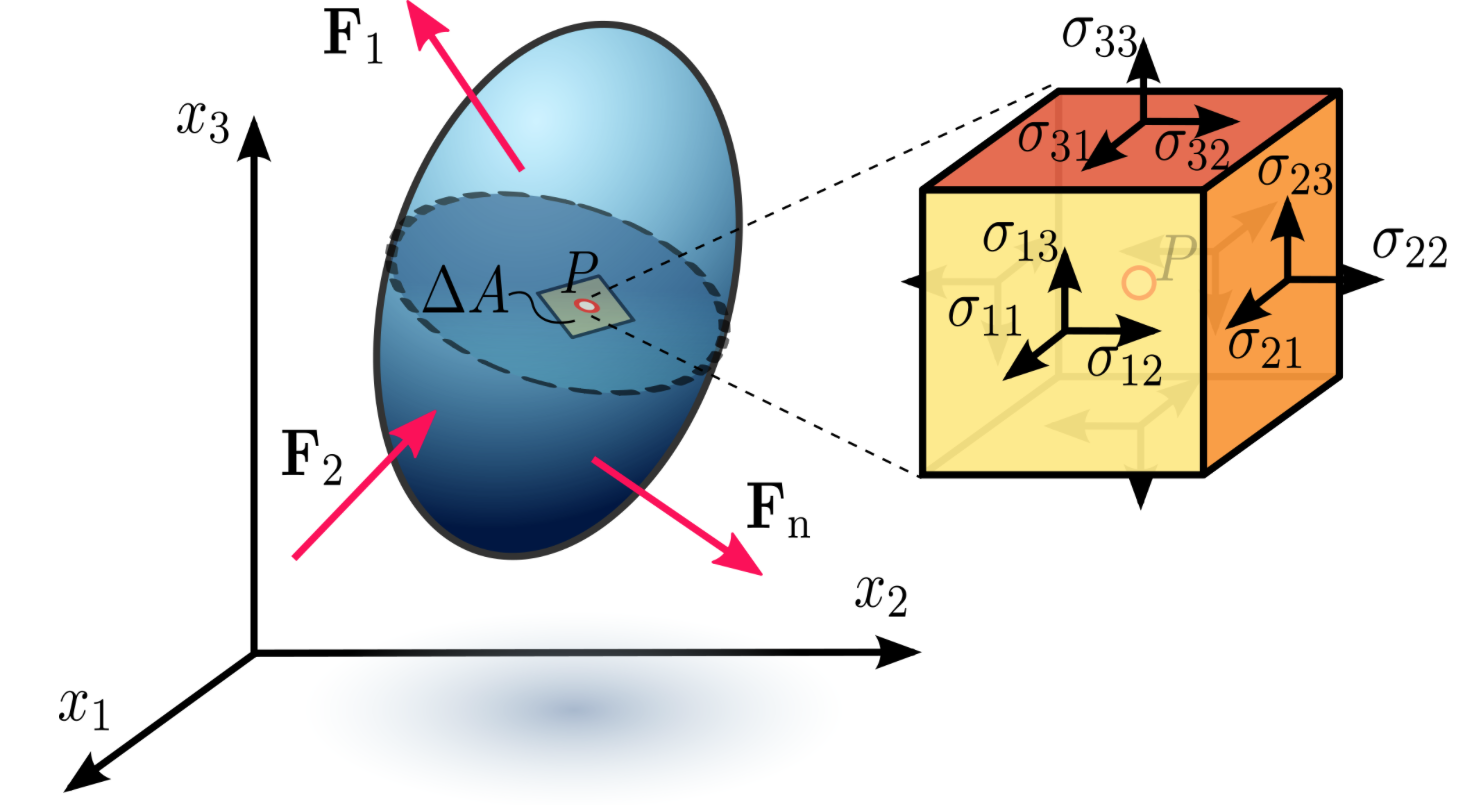
\includegraphics[width=0.75\textwidth]{figs/intro/Sigmas}
		\caption{Esfuerzos en un punto}
		\label{Sigmas}
	\end{figure}
	
	\begin{equation}
		\bm{\sigma} \coloneqq \begin{bmatrix}
			\sigma_{11} & \sigma_{12} & \sigma_{13} \\
			\sigma_{21} & \sigma_{22} & \sigma_{23} \\
			\sigma_{31} & \sigma_{32} & \sigma_{33}
		\end{bmatrix} = \begin{bmatrix}
			\sigma_x & \tau_{xy} & \tau_{xz} \\
			\tau_{yx} & \sigma_y & \tau_{yz} \\
			\tau_{zx} & \tau_{zy} & \sigma_z
		\end{bmatrix}
		\label{CauchyTensor}
	\end{equation}
\marginnote[-1.2cm]{\small Tensor de esfuerzos de Cauchy}
	
	Se utiliza la correspondencia siguiente:
	\begin{equation*}
		\begin{array}{ccc}
			x_1 \rightarrow x; & x_2 \rightarrow y; & x_3 \rightarrow z
		\end{array}
	\end{equation*}
	
	El tensor de esfuerzos de Cauchy es simétrico, esta simetría permite escribirlo en formato vectorial:
	\begin{equation}
	    \underline{\bm{\sigma}} = \begin{bmatrix} \sigma_x & \sigma_y & \sigma_z & \tau_{yz} & \tau_{xz} & \tau_{zy} \end{bmatrix}^T
	\end{equation}
	
	aplicado a pórticos planos se reduce a:
	\begin{equation}
	    \underline{\bm{\sigma}} = \begin{bmatrix} \sigma_{x} & \sigma_{y} & \tau_{xy} \end{bmatrix}
	\end{equation}
	
	en problemas unidimensionales:
	\begin{equation}
	    \underline{\bm{\sigma}} = \sigma_x
	\end{equation}

En general, para un problema tridimensional $\bm{\sigma} \in \mathbb{R}^6$, en el caso bidimensional $\bm{\sigma} \in \mathbb{R}^3$ y, en problemas unidimensionales $\bm{\sigma} \in \mathbb{R}$.

\subsection{Vector de tracción de Cauchy}
	
	\index{Vector de tracción de Cauchy}
	Observando ahora la fig. \ref{fig:TetraCauchy} y la fig. \ref{Sigmas} anterior, se puede demostrar sin dificultad la siguiente relación entre \textit{vector de tracción de Cauchy} $\mathbf{T}$ y  el \textit{tensor de esfuerzos de Cauchy} $\bm{\sigma}$:
	
	\marginpar{
\captionsetup{type=figure}
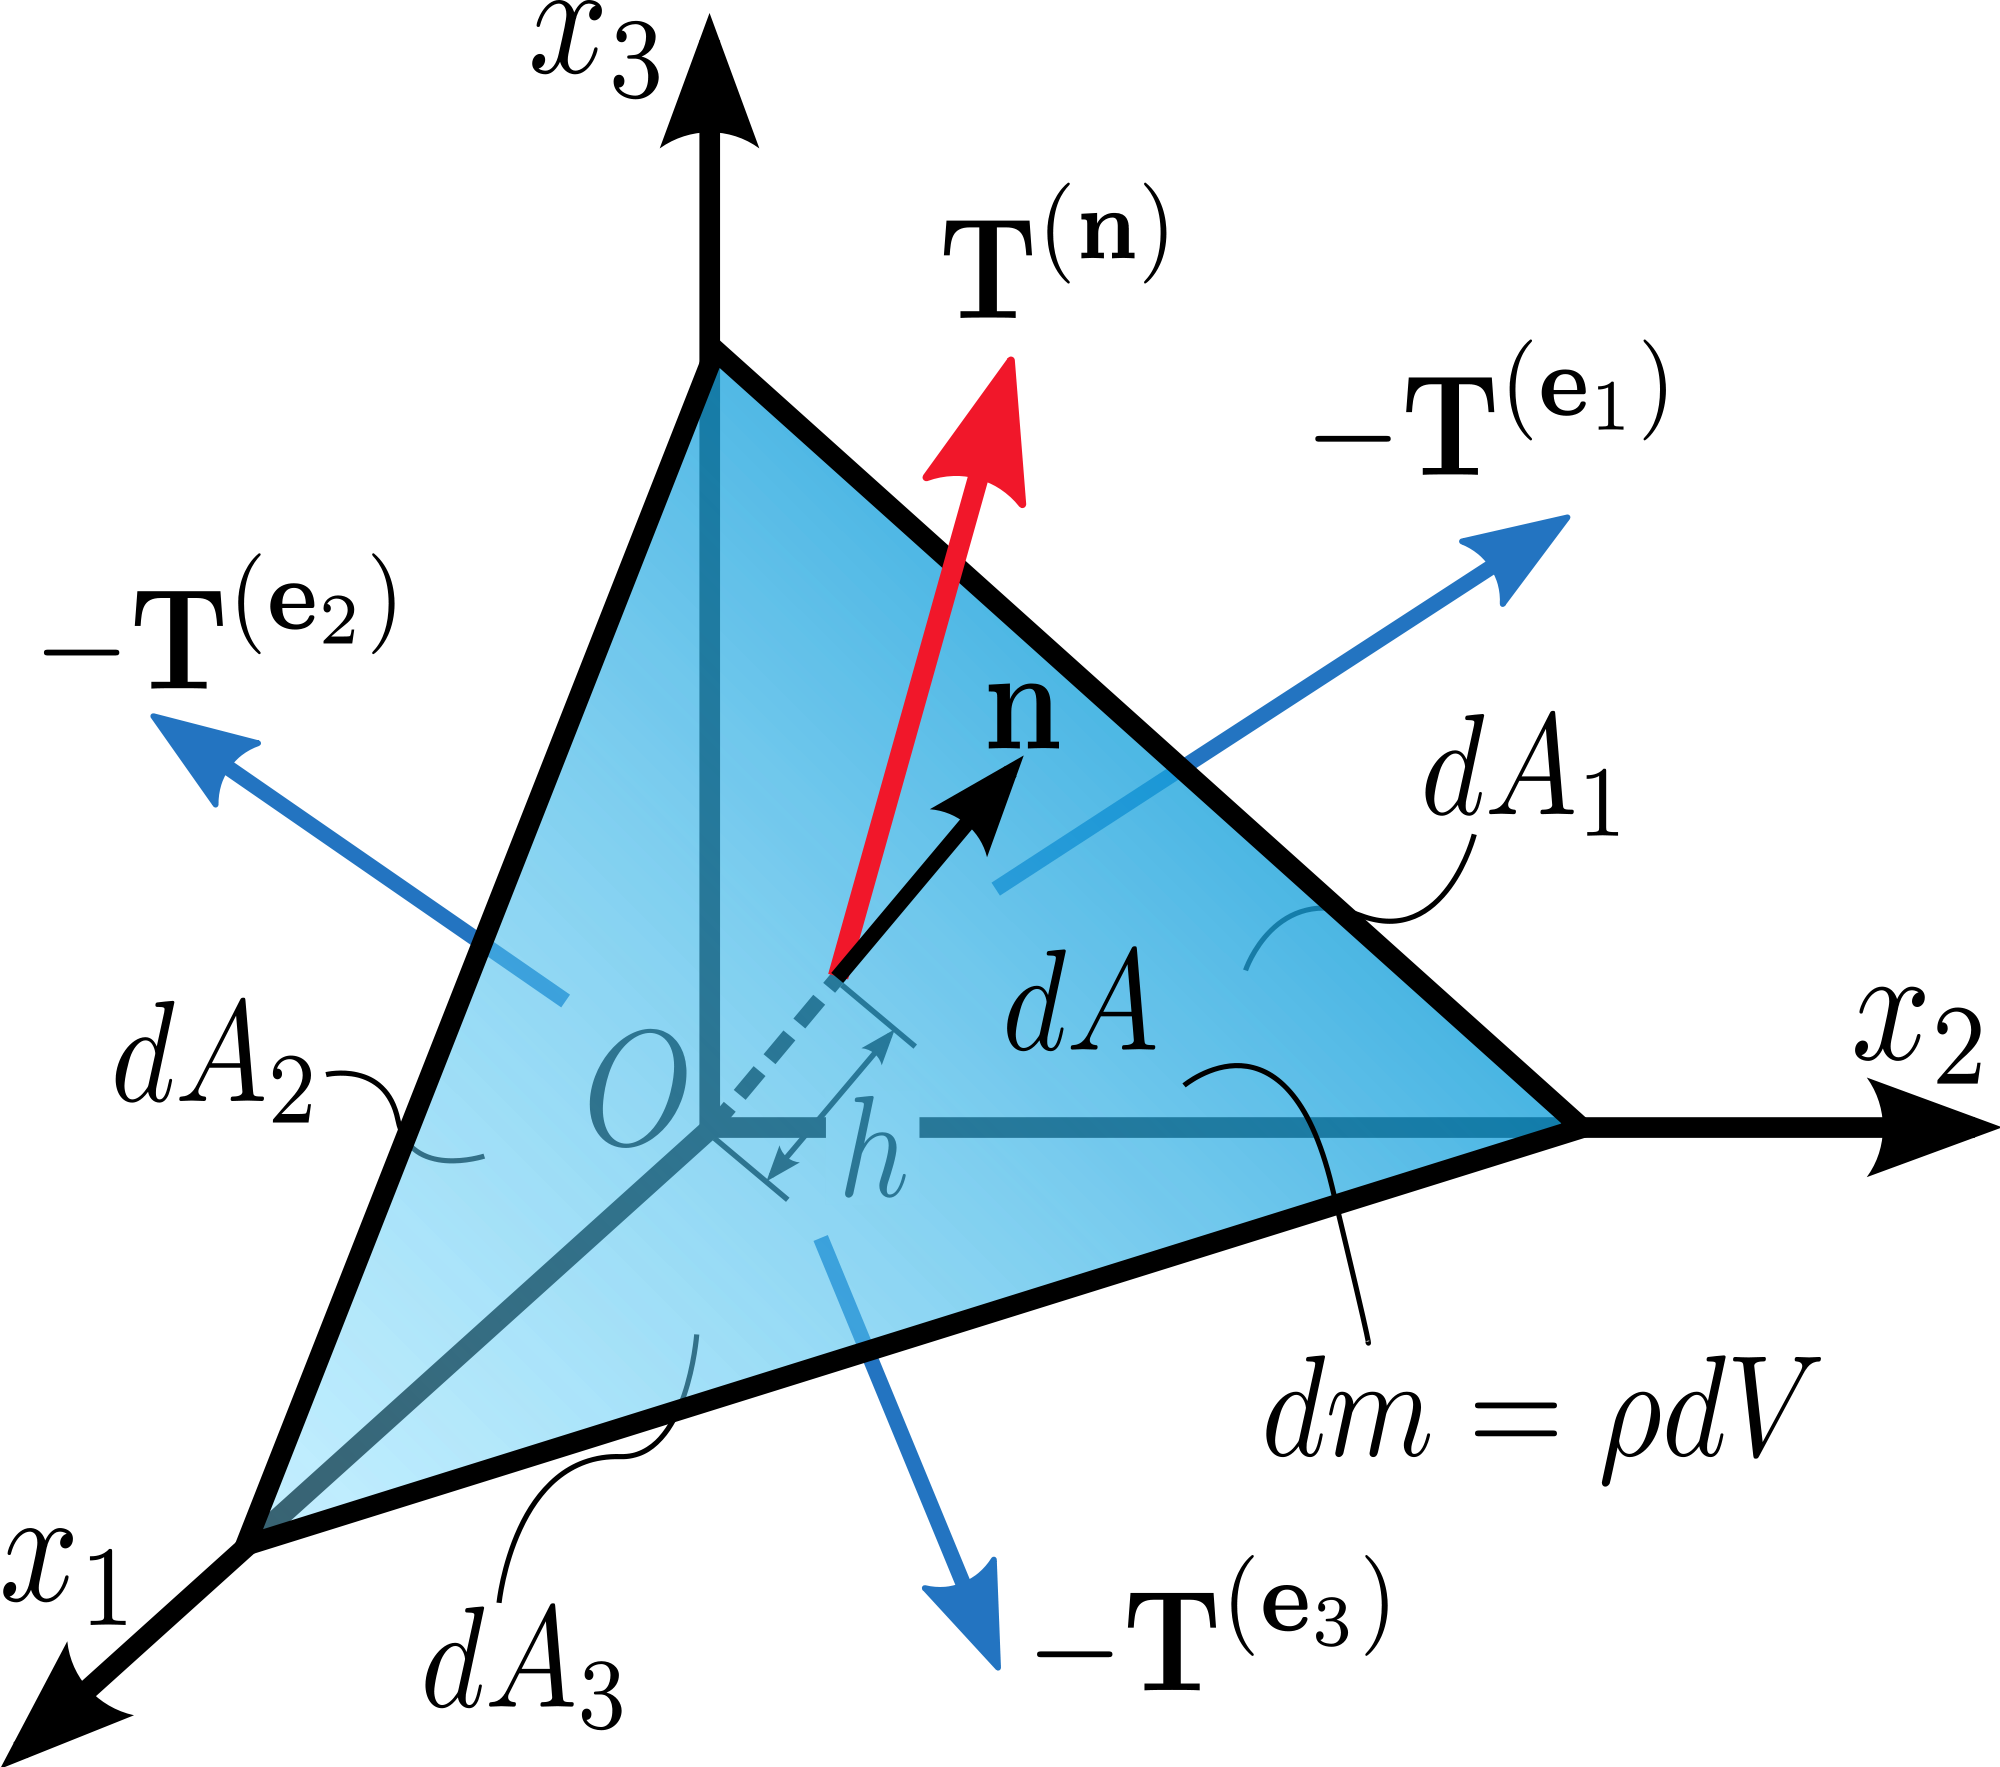
\includegraphics[width=\marginparwidth]{figs/intro/TetraCauchy}
\caption{Tetraedro de Cauchy}
\label{fig:TetraCauchy}
}
	
	\begin{equation}
		\begin{array}{c}
			\mathbf{T} = 
			\begin{bmatrix}
				T_1 ^{(\mathbf{n})} \\ T_2 ^{(\mathbf{n})} \\ T_3 ^{(\mathbf{n})}
			\end{bmatrix} = \begin{bmatrix}
			\sigma_x & \tau_{xy} & \tau_{xz} \\
			\tau_{yx} & \sigma_y & \tau_{yz} \\
			\tau_{zx} & \tau_{zy} & \sigma_z
		\end{bmatrix} \begin{bmatrix}
				n_1 \\ n_2 \\ n_3
			\end{bmatrix} \\ \\
			\boxed{\mathbf{T} = \bm{\sigma} \mathbf{n}}
		\end{array}
		\label{eq:tSigma}
	\end{equation}
	
	%%%%%%%%%%%%%%%%%%%%%%%
\subsection{Movimiento de un cuerpo}

\marginpar{
	\captionsetup{type=figure}
	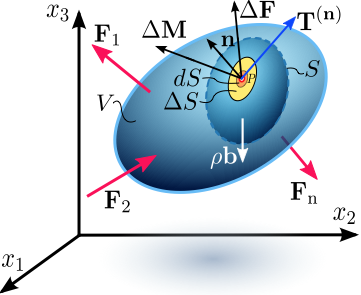
\includegraphics[width=\marginparwidth]{figs/intro/FuerzasCuerpo}
	\caption{Fuerzas sobre un cuerpo}
	\label{fig:FuerzasCuerpo}
\label{FuerzasCuerpo}
}
	
	Atendiendo la figura \ref{fig:FuerzasCuerpo} en donde se indican las fuerzas de superficie \index{fuerzas de superficie} 	$\mathbf{T}$ y las de cuerpo $\rho \mathbf{b}$, siendo $\rho$ la densidad del cuerpo en el punto $P$ y $\mathbf{b}$ la fuerza de cuerpo en $P$ por unidad de masa, puede escribirse las ecuaciones del movimiento, considerando la \textit{segunda Ley de Newton} sobre cada partícula que conforma el cuerpo y sumando en  todo el volumen, resulta así la siguiente
	ecuación\sidenote{Esta ecuación es además equivalente al teorema del impulso y la cantidad de movimiento lineal.}:
	
	\begin{equation}
		\int_S \mathbf{T} \, dS + \int_V \rho \mathbf{b} \, dV
		= \int_V \rho \mathbf{a} \, dV
	\end{equation}
	
	en la cual $\mathbf{a}$ es la aceleración de la partícula que ocupa el volumen $dV$.
	
	En la primera integral podemos sustituir $\mathbf{T}$
	por $\bm{\sigma} \mathbf{n}$ según lo visto en \eqref{eq:tSigma}
	
	\begin{equation}
		\int_S \bm{\sigma} \mathbf{n} \, dS + \int_V \rho \mathbf{b} \, dV
		= \int_V \rho \mathbf{a} \, dV
		\label{eq:parcial}
	\end{equation}
	
	Recordamos el \textit{teorema de Gauss}\index{teorema de Gauss} que posibilita substituir una integral de superficie por otra de volumen:
	
	\begin{equation}
		\int_S \bm{\sigma} \mathbf{n} \, dS = \int_V \nabla
		\bm{\sigma} \, dV
		\label{Gauss}
	\end{equation}
\marginnote[-.9cm]{\small Teorema de Gauss}

En donde: $\nabla = \begin{bmatrix}
	\dfrac{\partial}{\partial x} & \dfrac{\partial}{\partial y} & \dfrac{\partial}{\partial z}
\end{bmatrix}$ es el operador nabla.
	
	Usando \eqref{Gauss} en \eqref{eq:parcial} llegamos a
	\begin{equation}
		\int_V \left( \nabla \bm{\sigma}  + \rho \mathbf{b} - \rho
		\mathbf{a} \right) \, dV = \mathbf{0}
	\end{equation}
	
	como el volumen $V$ es arbitrario, se debe cumplir que:
	\begin{equation}
		\nabla \bm{\sigma} + \rho \mathbf{b} = \rho \mathbf{a}
		\label{mov1}
	\end{equation}
\marginnote[-.85cm]{\small Ecuación de movimiento}
	
	%%%%%%%%%%%%%%%%%%%
	\subsection{Ecuaciones de equilibrio}
	
	En el equilibrio, es decir, si el cuerpo está en reposo o con velocidad constante, la aceleración es nula $\mathbf{a} = \mathbf{0}$. Además si se llama $\mathbf{f} = \rho \mathbf{b}$ a la fuerza de cuerpo por unidad de volumen, entonces:
	
	\begin{equation}
		\boxed{\nabla \bm{\sigma} + \mathbf{f} = \mathbf{0}}
		\label{eq:equil}
	\end{equation}
	\marginnote[-.65cm]{\small Ecuación de equilibrio}
	
	Ya que el tensor de esfuerzos de Cauchy es simétrico, las \textit{ecuaciones de equilibrio} se pueden escribir, en su forma extendida:
	\begin{equation}
		\begin{array}{c}
			\dfrac{\partial \sigma_{x}}{\partial x} + \dfrac{\partial
				\tau_{xy}}{\partial y} + \dfrac{\partial \tau_{xz}}{\partial
				z} + f_x = 0 \\ \\
			\dfrac{\partial \tau_{xy}}{\partial y} + \dfrac{\partial
				\sigma_{y}}{\partial y} + \dfrac{\partial \tau_{yz}}{\partial
				z} + f_y = 0 \\ \\
			\dfrac{\partial \tau_{xz}}{\partial x} + \dfrac{\partial
				\tau_{yz}}{\partial y} + \dfrac{\partial \sigma_{z}}{\partial
				z} + f_z =0
		\end{array}
	\end{equation}
	
	Esta es la ``forma fuerte''\index{forma fuerte} de las ecuaciones diferenciales parciales de equilibrio.
	
\section{Deformación unitaria}
\index{Deformación unitaria}

\subsection{Desplazamiento}
\index{Desplazamiento}

Considere un punto material, de una estructura cualquiera, en la posición $\mathbf{r} = \begin{bmatrix}
	x & y & z
\end{bmatrix}^T $ de un sistema de coordenadas $xyz$ el cual se muestra en la fig. \ref{fig:desplaz}. Luego de la acción de las fuerzas el punto material sufre un desplazamiento $\mathbf{u} = \begin{bmatrix}
u & v & w
\end{bmatrix}^T$ y se ubica en $\mathbf{s} = \begin{bmatrix}
x + u & y + v & z + w
\end{bmatrix}^T$.

\begin{figure}[ht]
	\centering
	\begin{tikzpicture}[scale=1]
		\draw[-latex] (-1, 0, 0) -- (5, 0, 0) node[below left]{$x$};
		\draw[-latex] (0, -1, 0) -- (0, 5, 0) node[left]{$y$};
		\draw[-latex] (0, 0, -1) -- (0, 0, 5) node[left]{$z$};
		
		\coordinate (o) at (0, 0, 0);
		\coordinate (r) at (2, 3, 1);
		\coordinate (u) at (2, -1, 0);
		\coordinate (s) at ($(r)+(u)$);
		\coordinate (dr) at (-1, 1, -1);
		\coordinate (rdr) at ($(r) + (dr)$);
		
		\draw[thick, -latex, red] (o) -- (r) node[left, pos=.7]{$\mathbf{r}$};
		\draw[thick, -latex, blue] (r) -- (s) node[below, pos=.47]{$\mathbf{u}(\mathbf{r})$};
		\draw[thick, -latex, red] (o) -- (s) node[above, pos=.5]{$\mathbf{s}$};
		\draw[thick, -latex, red] (o) -- (rdr) node[above, pos=.7, rotate=76]{$\mathbf{r} + \Delta \mathbf{r}$};
		\draw[thick, -latex, blue] (r) -- (rdr) node[left, pos=.25]{$\Delta \mathbf{r}$};
		\draw[thick, -latex, red] (o) -- ($(s)+(dr)$) node[above, rotate=47, pos=.6]{$\mathbf{r} + \Delta \mathbf{s}$};
		\draw[thick, -latex, blue] (s) -- ($(s)+(dr)$) node[right, pos=.5]{$\Delta \mathbf{s}$};
		\draw[thick, -latex, blue] (rdr) -- ($(rdr)+(u)$) node[above, pos=.5, rotate=-27]{$\Delta \mathbf{u}(\mathbf{r} + \Delta \mathbf{r})$};
	\end{tikzpicture}
\caption{Desplazamiento}
\label{fig:desplaz}
\end{figure}

Ahora considere una partícula vecina en la posición $\mathbf{r} + \Delta \mathbf{r}$. En la configuración desplazada, la nueva posición de este punto será:
\begin{equation}
	\mathbf{s} + \Delta \mathbf{s} = \mathbf{r} + \Delta \mathbf{r} + \mathbf{u}(\mathbf{r} + \Delta \mathbf{r})
\end{equation}

por lo tanto (ver fig. \ref{fig:desplaz}):
\begin{equation}
	\Delta \mathbf{s} = \Delta \mathbf{r} + \mathbf{u}(\mathbf{r} + \Delta \mathbf{r}) - \mathbf{u}(\mathbf{r})
	\label{eq:ese}
\end{equation}
	
Si $\Delta \mathbf{u} = \mathbf{u}(\mathbf{r} + \Delta \mathbf{r}) - \mathbf{u}(\mathbf{r})$ es suficientemente pequeño:
\begin{equation}
	\begin{split}
	\Delta\mathbf{u} = \begin{bmatrix}
		\Delta u \\ \Delta v \\ \Delta w
	\end{bmatrix} & \approx \begin{bmatrix}
		\dfrac{\partial u}{\partial x} \Delta x + \dfrac{\partial u}{\partial y} \Delta y + \dfrac{\partial u}{\partial z} \Delta z \\[5mm]
		\dfrac{\partial v}{\partial x} \Delta x + \dfrac{\partial v}{\partial y} \Delta y + \dfrac{\partial v}{\partial z} \Delta z \\[5mm]
		\dfrac{\partial w}{\partial x} \Delta x + \dfrac{\partial w}{\partial y} \Delta y + \dfrac{\partial w}{\partial z} \Delta z
	\end{bmatrix} = \begin{bmatrix}
	\dfrac{\partial u}{\partial x} & \dfrac{\partial u}{\partial y} & \dfrac{\partial u}{\partial z} \\[5mm]
	\dfrac{\partial v}{\partial x} & \dfrac{\partial v}{\partial y} & \dfrac{\partial v}{\partial z} \\[5mm]
	\dfrac{\partial w}{\partial x} & \dfrac{\partial w}{\partial y} & \dfrac{\partial w}{\partial z}
\end{bmatrix} \begin{bmatrix}
\Delta x \\ \Delta y \\ \Delta z
\end{bmatrix} \\[5mm] &= \bm{\alpha} \Delta \mathbf{r}
\end{split}
\label{eq:Delta_u}
\end{equation}

En donde:
\begin{equation}
	\bm{\alpha} \coloneqq \begin{bmatrix}
		\dfrac{\partial u}{\partial x} & \dfrac{\partial u}{\partial y} & \dfrac{\partial u}{\partial z} \\[5mm]
		\dfrac{\partial v}{\partial x} & \dfrac{\partial v}{\partial y} & \dfrac{\partial v}{\partial z} \\[5mm]
		\dfrac{\partial w}{\partial x} & \dfrac{\partial w}{\partial y} & \dfrac{\partial w}{\partial z}
	\end{bmatrix} = \left( \nabla \mathbf{u}^T \right)^T
\end{equation}

Se observa de \eqref{eq:ese} y \eqref{eq:Delta_u} que:

\begin{equation}
	\Delta \mathbf{s} = \left( \mathbf{I} + \bm{\alpha} \right) \Delta \mathbf{r}
	\label{eq:Delta_s}
\end{equation}

\subsection{Tensor deformación unitaria}
\index{Tensor deformación unitaria}
A continuación se calcula la norma del vector $\Delta \mathbf{s}$ dado por \eqref{eq:Delta_s}, que en un entorno infinitesimal será:

\begin{equation}
	|| d \mathbf{s} ||^2 = \left(d \mathbf{s}\right)^T d \mathbf{s} = \left(d \mathbf{r}\right)^T \left( \mathbf{I} + \bm{\alpha}^T \right) \left( \mathbf{I} + \bm{\alpha} \right) d \mathbf{r} = \left(d \mathbf{r}\right)^T \left(\mathbf{I} + 2 \mathbf{E} \right) d \mathbf{r}
\end{equation}

En donde:
\begin{equation}
	\mathbf{E} = \dfrac{1}{2} \left(\bm{\alpha} + \bm{\alpha}^T + \bm{\alpha}\bm{\alpha}^T \right)
\end{equation}
\marginnote[-1cm]{\small Tensor deformación unitaria de Green - Saint-Venant}

Notar que $\mathbf{E}$ es un tensor simétrico.

Despreciando en $\mathbf{E}$, el término de segundo orden, se obtiene el tensor (simétrico) deformación unitaria que se define como:

\begin{equation}
	\begin{split}
		\bm{\varepsilon} & \coloneqq \dfrac{1}{2} \left(\bm{\alpha} + \bm{\alpha}^T \right) \\ &=  \begin{bmatrix}
		\dfrac{\partial u}{\partial x} & \dfrac{1}{2} \left(\dfrac{\partial u}{\partial y} + \dfrac{\partial v}{\partial x}\right) & \dfrac{1}{2} \left(\dfrac{\partial u}{\partial z} + \dfrac{\partial w}{\partial x}\right) \\[5mm]
		\dfrac{1}{2} \left(\dfrac{\partial v}{\partial x} + \dfrac{\partial u}{\partial y}\right) & \dfrac{\partial v}{\partial y} & \dfrac{1}{2} \left(\dfrac{\partial v}{\partial z} + \dfrac{\partial w}{\partial y}\right) \\[5mm]
		\dfrac{1}{2} \left(\dfrac{\partial w}{\partial x} + \dfrac{\partial u}{\partial z}\right) & \dfrac{1}{2} \left(\dfrac{\partial w}{\partial y} + \dfrac{\partial v}{\partial z}\right) & \dfrac{\partial w}{\partial z}
	\end{bmatrix}
	\end{split}
\end{equation}

de donde:
\begin{equation}
	\bm{\varepsilon} = \begin{bmatrix}
		\varepsilon_{11} & \varepsilon_{12} & \varepsilon_{13} \\
		\varepsilon_{21} & \varepsilon_{22} & \varepsilon_{23} \\
		\varepsilon_{31} & \varepsilon_{32} & \varepsilon_{33}
	\end{bmatrix} = \begin{bmatrix}
		\varepsilon_x & \dfrac{1}{2} \gamma_{xy} & \dfrac{1}{2} \gamma_{xz} \\[5mm]
		\dfrac{1}{2} \gamma_{yx} & \varepsilon_y & \dfrac{1}{2} \gamma_{yz} \\[5mm]
		\varepsilon_x & \dfrac{1}{2} \gamma_{xy} & \varepsilon_z \\
	\end{bmatrix}
\end{equation}

Es fácil ver que este tensor es simétrico, por lo que $\gamma_{ij} = \gamma_{ji}$. Debido a este hecho se puede definir el \textit{vector deformación unitaria}:

\begin{equation}
	\underline{\bm{\varepsilon}} \coloneqq \begin{bmatrix}
		\varepsilon_x & \varepsilon_y & \varepsilon_z & \gamma_{yz} & \gamma_{xz} & \gamma_{xy}
	\end{bmatrix}^T
\end{equation}

\section{Relaciones constitutivas}

Se supone un material elástico lineal, homogéneo e isotrópico. En este caso son necesarias dos constantes para relacionar linealmente las tensiones con las deformaciones unitarias.

\subsection{Constantes de Lamé}
\index{Constantes de Lamé}
La propuesta de relación lineal que define las constantes de Lamé\sidenote{Gabriel Lamé, francés (22 Julio 1795 – 1 Mayo 1870)} $\mu$ y $\lambda$, es:

\begin{equation}
	\bm{\sigma} = 2 \mu \bm{\varepsilon} + \lambda \mathsf{tr} \left( \bm{\varepsilon} \right) \mathbf{I}
\end{equation}

\subsection{Ley de Hooke}
\index{Ley de Hooke}
En ingeniería es más usual, utilizar la ley de Hooke\sidenote{Robert Hooke, inglés (18 Julio 1635 – 3 Marzo 1703)}, con las constantes $E$ y $\nu$, que son respectivamente el módulo de elasticidad o de Young\sidenote{Thomas Young, inglés (13 Junio 1773 – 10 Mayo 1829)} y el módulo de Poisson\sidenote{Siméon Denis Poisson, francés (21 Junio 1781 – 25 Abril 1840)}.

\begin{equation}
	\begin{split}
		\varepsilon_x &= \dfrac{\sigma_x}{E} - \nu \dfrac{\sigma_y}{E} - \nu \dfrac{\sigma_z}{E}\\[5mm]
		\varepsilon_x &= -\nu \dfrac{\sigma_x}{E} + \dfrac{\sigma_y}{E} - \nu \dfrac{\sigma_z}{E}\\[5mm]
		\varepsilon_x &= -\nu \dfrac{\sigma_x}{E} - \nu \dfrac{\sigma_y}{E} + \dfrac{\sigma_z}{E}\\[5mm]
		\gamma_{yz} &= \dfrac{\tau_{yz}}{G}; \quad \gamma_{xz} = \dfrac{\tau_{xz}}{G} \quad
		\gamma_{xy} = \dfrac{\tau_{xy}}{G}
	\end{split}
\end{equation}

En donde, el módulo de corte $G = \dfrac{E}{2 (1 + \nu)}$

Con los vectores $\bm{\sigma}$ y $\bm{\varepsilon}$, la relación anterior, matricialmente, se puede escribir:

\begin{equation}
	\underline{\bm{\sigma}} = \mathbf{D} \underline{\bm{\varepsilon}}
\end{equation}

En donde, $\mathbf{D}$ es una matriz simétrica $6 \times 6$.

\begin{equation}
	\mathbf{D} = \dfrac{E}{(1+\nu)(1-2\nu)}
	\begin{bmatrix}
		1-\nu & \nu & \nu & 0 & 0 & 0 \\
		\nu & 1-\nu & \nu & 0 & 0 & 0 \\
		\nu & \nu & 1-\nu & 0 & 0 & 0 \\
		0 & 0 & 0 & 0.5-2\nu & 0 & 0 \\
		0 & 0 & 0 & 0 & 0.5-2\nu & 0 \\
		0 & 0 & 0 & 0 & 0 & 0.5-2\nu
	\end{bmatrix}
\end{equation}


\subsection{Energía potencial total}

La energía potencial total\index{energía potencial total} del sistema estructural se define como:

\begin{equation}
	\Pi = U + W
	\label{eq:EP}
\end{equation}

Siendo $U$ la energía de deformación unitaria\index{energía de deformación unitaria} y $W$ el potencial de trabajo\index{potencial de trabajo}. La energía de deformación unitaria es:

\begin{equation}
	U = \dfrac{1}{2} \int_V \underline{\bm{\sigma}}^T \underline{\bm{\varepsilon}} \, dV
\end{equation}

El potencial de trabajo está dado por:

\begin{equation}
	W = -\int_V \mathbf{u}^T \mathbf{f} \, dV - \int_S \mathbf{u}^T \mathbf{T} \, dS - \sum_i \mathbf{u}^T_i \mathbf{P}_i
\end{equation}


\index{Principio de mínima energía potencial}

\begin{kaobox}[frametitle=Principio de mínima energía potencial]
	Para sistemas conservativos, de todos los campos de desplazamientos cinemáticamente admisibles, aquellos que corresponden a condiciones de equilibrio, extremizan la energía potencial total. Si la condición extrema es un mínimo, el estado de equilibrio es estable
\end{kaobox}

\section{Energía y ecuaciones de campo de elementos estructurales}

\subsection{Barra con carga axial}

En la fig. \ref{fig:barra-carga-axial} se muestra una barra de sección variable con carga axial, su ecuación diferencial gobernante es:
\begin{equation}
	\dfrac{d}{dx} \left( AE \dfrac{du}{dx} \right) + p = 0
	\label{eq:barra-axial}
\end{equation}

\marginpar{
	\captionsetup{type=figure}
	\includestandalone[width=\marginparwidth]{figs/fundamentales/barra-carga-axial}
	\caption{Barra con carga axial}
	\label{fig:barra-carga-axial}
}

Si $AE = cte.$ \eqref{eq:barra-axial} se convierte en:
\begin{equation}
	AE \dfrac{d^2u}{dx^2} + p = 0
\end{equation}

Por otro lado, la energía potencial total es:

\begin{equation}
	\Pi = \dfrac{1}{2} \int_L \sigma \varepsilon A \, dx - \int_L up\, dx - \sum_i u_i P_i
	\label{eq:energia_unidimensionales}
\end{equation}

como $\sigma A = EA \varepsilon = EA \dfrac{du}{dx}$, entonces:

\begin{equation}
	\Pi = \dfrac{1}{2} \int_L EA \left( \dfrac{du}{dx} \right)^2 \, dx - \int_L up\, dx - \sum_i u_i P_i
	\label{eq:eptuni}
\end{equation}

\subsection{Vigas}

La fig. \ref{fig:viga} muestra un caso particular de viga, en general la ecuación diferencial gobernante es:

\begin{equation}
	\dfrac{d^2}{dx^2} \left( EI \dfrac{d^2v}{dx^2}\right) - q = 0
	\label{eq:ed-viga}
\end{equation}

\marginpar{
	\captionsetup{type=figure}
	\includestandalone[width=\marginparwidth]{figs/fundamentales/viga0}
	\caption{Viga con carga distribuida.}
	\label{fig:viga}
}

Si $EI = cte.$ \eqref{eq:ed-viga} se convierte en:

\begin{equation}
	\dfrac{d^4v}{dx^4} - \dfrac{q}{EI} = 0
	\label{eq:ed-viga-cte}
\end{equation}

La energía potencial total es:
\begin{equation}
	\Pi = \frac{1}{2} \int_L EI \left(\frac{d^2v}{dx^2}\right)^2 \, dx - \int_L vq \, dx - \sum_i v_iP_i
	\label{eq:energia-vigas}
\end{equation}

en donde $v = v(x)$ es el campo de desplazamientos verticales de la viga, con carga 
distribuida $q = q(x)$ y puntuales $P_i$ (las cargas se consideran positivas hacia 
arriba, coherentes con el sentido positivo de $v$).

\subsection{Losas}

En la fig. \ref{fig:losa0}, se representa una losa cargada. La ecuación diferencial gobernante es \cite{timoshenko1959theory}:
\begin{equation}
	 \dfrac{\partial^4 w}{\partial x^4} + 2\dfrac{\partial^4 w}{\partial x^2y^2} + \dfrac{\partial^4 w}{\partial y^4} - \dfrac{q}{D} = 0
\end{equation}
\marginpar{
	\captionsetup{type=figure}
	\includestandalone[width=\marginparwidth]{figs/fundamentales/losa0}
	\caption{Losa cargada.}
	\label{fig:losa0}
}
con:
\begin{equation}
	D = \dfrac{Eh^3}{12 (1 - \nu^2)}
\end{equation}

O también:
\begin{equation}
	\laplace^2 w - \dfrac{q}{D} = 0
\end{equation}

en donde $\laplace (\cdot)$ es el operador de Laplace:
\begin{equation}
	\laplace (\cdot) = \nabla^2 (\cdot) = \dfrac{\partial^2 (\cdot)}{\partial x^2} + \dfrac{\partial^2 (\cdot)}{\partial y^2}
\end{equation}

La energía de deformación unitaria es:
\begin{equation}
	U = \frac{1}{2} \iint_S D \left[ \left( \frac{\partial^2 w}{\partial x^2} \right)^2 + 2 \frac{\partial^2 w}{\partial x^2} \frac{\partial^2 w}{\partial y^2} + \left( \frac{\partial^2 w}{\partial x^2} \right)^2 \right] \ dx dy
\end{equation}

Por lo tanto, la energía potencial total es:

\begin{equation}
	\Pi = \frac{1}{2} \iint_S D \left( \laplace^2 w \right)^2 \ dx dy - \iint_S w q \ dx dy
\end{equation}

	%!TEX root = ../main.tex
\setchapterimage[7.5cm]{figs/aproximados/domo}
\setchapterpreamble[u]{\margintoc}

\chapter{Métodos aproximados} \label{chap:aproximados}

\begin{kaobox}
	``Calidad significa hacerlo bien cuando nadie está mirando"
	
	``Una de las grandes sorpresas del hombre es encontrar que puede hacer lo que temía no podía hacer"
	\begin{flushright}
		Henry Ford
	\end{flushright}
\end{kaobox}

La incógnita maestra es el campo de desplazamientos $\mathbf{u}$, los métodos aproximados, en general, se basan en suponer un campo de desplazamientos $\tilde{\mathbf{u}}$ y aplicar algunos criterios para aproximarlo a la solución exacta $\mathbf{u}$ lo mejor posible.

\section{Método de Rayleigh-Ritz}

En el presente método se realiza la construcción del campo de desplazamientos $\tilde{\mathbf{u}} = \begin{bmatrix}
	\tilde{u} & \tilde{v} & \tilde{w}
\end{bmatrix}^T$ como combinación lineal de ciertas funciones:

\marginnote[2cm]{$n > m > l$}
\begin{equation}
	\begin{split}
		\tilde{u}(x, y, z) = \sum_i a_i \phi_i(x, y, z) & \qquad \forall \ i = 0, \dots, l-1\\
		\tilde{v}(x, y, z) = \sum_j a_j \phi_j(x, y, z) & \qquad \forall \ j = l, \dots, m - 1 \\
		\tilde{w}(x, y, z) = \sum_k a_k \phi_k(x, y, z) & \qquad \forall \ k = m, \dots, n - 1
	\end{split}
\end{equation}

Las $n$ funciones $\phi_i(x, y, z)$ usualmente son polinomios. Los desplazamientos $\tilde{\mathbf{u}}$ necesitan satisfacer \textit{solo las condiciones esenciales} de frontera.
\marginnote[]{Las funciones de aproximación deben satisfacer solo las condiciones esenciales de frontera}

Con estas funciones aproximadas la energía potencial \eqref{eq:EP} se convierte en:

\begin{equation}
	\Pi = \Pi(a_0, a_1, \dots a_{r-1})
\end{equation}

En donde $r$ es el número de incógnitas independientes.

De acuerdo al principio de mínima energía potencial, se debe cumplir:

\begin{equation}
	\dfrac{\partial \Pi}{\partial a_i} = 0 \qquad \forall \; i = 0, \dots, r - 1
\end{equation}

\begin{example}
	Calcule el campo de desplazamientos para la barra de la fig. \ref{fig:BarraVertical}, utilizando el método de Rayleigh-Ritz. Datos de la barra: densidad $\rho$, módulo de elasticidad $E$, sección transversal $A$, longitud $L$.
	
	
	\begin{marginfigure}[-1cm]
		\centering
		\includestandalone[width=.4\textwidth]{figs/aproximados/barra0}
		\caption{Barra vertical bajo acción de la gravedad.}
		\label{fig:BarraVertical}
	\end{marginfigure}
	
	\textit{Solución}:
	\vspace{2mm}
	
	Se supone:
	\begin{equation}
		u(x) = a_0 + a_1 x + a_2 x^2
	\end{equation}
	que debe cumplir las condiciones esenciales de frontera:
	
	\begin{equation}
		\begin{cases}
			u(0) = 0 \implies a_0 = 0 \\
			u(L) = 0 \implies a_2 = -\dfrac{a_1}{L}
		\end{cases}
	\end{equation}
	
	entonces:
	\begin{equation}
		u(x) = a_1 x \left(1 - \dfrac{x}{L}\right)
		\label{eq:rr1}
	\end{equation}
	
	cuya derivada es:
	\begin{equation}
		\dfrac{du}{dx} = a_1 \left( 1 - \dfrac{2}{L}x \right)
		\label{eq:der1}
	\end{equation}
	
	Según \eqref{eq:eptuni}, la energía potencial total es:
	\begin{equation*}
		\Pi = \dfrac{1}{2} \int_L EA \left( \dfrac{du}{dx} \right)^2 \, dx - \int_L up\, dx - \sum_i u_i P_i
	\end{equation*}
	
	en este caso, la carga por unidad de longitud $p = A \rho g$ y no existen cargas puntuales, es decir: $P_i = 0$.
	
	Substituyendo \eqref{eq:der1} en la expresión de la energía potencial y haciendo,
	\begin{equation*}
		\dfrac{\partial \Pi}{\partial a_1} = 0 
	\end{equation*}
	
	
	se obtiene el resultado deseado:
	\begin{equation}
		u(x) = \dfrac{\rho g L}{2E} x \left(1 - \dfrac{x}{L}\right)
		\label{eq:rr2}
	\end{equation}
\end{example}

\section{Método de residuos ponderados}

Básicamente son métodos para resolver ecuaciones diferenciales.

La idea parte de recordar que, en un sistema de ecuaciones lineales $\mathbf{Ax} = \mathbf{b}$, si $\mathbf{b} \not \in C(\mathbf{A})$, siendo $\mathbf{p}$ el vector proyección de $\mathbf{b}$ sobre el espacio columna $C(\mathbf{A})$, el vector error o \textit{residuo} $\bm{\epsilon} = \mathbf{b} - \mathbf{p}$ es ortogonal a $C(\mathbf{A})$ y por lo tanto pertenece al espacio nulo izquierdo, es decir $\bm{\epsilon} \in N(\mathbf{A}^T)$, ya que $C(\mathbf{A})^{\perp} = N(\mathbf{A}^T)$, entonces:
\begin{equation}
	\mathbf{A}^T \mathbf{y} = \mathbf{0}
	\label{eq:residuo}
\end{equation}

Se extienden estas ideas al espacio de Hilbert\sidenote{David Hilbert, alemán (23 Enero 1862 – 14 Febrero 1943)}. Suponga $\mathbf{y} \rightarrow \bm{\epsilon}$ y que la ecuación diferencial del problema sea:
\begin{equation}
	L \mathbf{u} = \mathbf{P}
	\label{eq:LuP}
\end{equation}
En donde $L$ es un operador diferencial y $\mathbf{P}$ una función vectorial.

Si se aproxima el campo vectorial $\mathbf{u}$ con $\tilde{\mathbf{u}}$, la solución ya no es exacta, habrá un residuo, el cual será:
\begin{equation}
	\bm{\epsilon} = L \tilde{\mathbf{u}} - \mathbf{P}
\end{equation}

Las funciones de aproximación $\tilde{\mathbf{u}}$ deben cumplir con \textit{todas} las condiciones de frontera, esenciales y naturales.\marginnote[]{Las funciones aproximadoras, en los métodos de residuos ponderados, deben cumplir con todas las condiciones de frontera.}

Entonces \eqref{eq:residuo} se convierte en:
\begin{equation}
	\int_V \mathbf{w}^T \bm{\varepsilon} \, dV = 0
	\label{eq:pond}
\end{equation}

La elección de $\mathbf{w}$ lleva a diferentes métodos de resolución, un par de ellos son el método de mínimos cuadrados y el de Galerkin\sidenote{Boris Grigoryevich Galerkin, ruso (4 Marzo 1871 – 12 Julio 1945)}.

\subsection{Mínimos cuadrados}
Se trata de minimizar la suma de los cuadrados de los errores, en este contexto la expresión matemática es:
\begin{equation}
	\min S: \quad S = \int_V ||\bm{\varepsilon}||^2 \, dV =  \int_V \bm{\epsilon}^T \bm{\epsilon} \, dV
\end{equation}

si $\tilde{\mathbf{u}}$ depende de parámetros $a_i$, entonces:
\begin{equation}
	\dfrac{\partial S}{\partial a_i} = 2 \int_V \bm{\epsilon}^T \dfrac{\partial \bm{\epsilon}}{\partial a_i} \, dV = 0
\end{equation}

es decir, las funciones ponderadoras son las derivadas del residual:
\begin{equation}
	\boxed{\int_V \bm{\epsilon}^T \dfrac{\partial \bm{\epsilon}}{\partial a_i} \, dV = 0}
\end{equation}

Para casos unidimensionales en barras de sección constante:
\begin{equation}
	\int_L \epsilon \dfrac{\partial \epsilon}{\partial a_i} \, dx = 0
	\label{eq:min2}
\end{equation}

\begin{exercise}
	Calcule el campo de desplazamientos para la barra de la \reffig{BarraVertical}, utilizando el método de los mínimos cuadrados. Datos de la barra: densidad $\rho$, módulo de elasticidad $E$, sección transversal $A$, longitud $L$.
	
	\begin{marginfigure}[-.5cm]
		\centering
		\includestandalone[width=.4\textwidth]{figs/aproximados/barra0}
		\repeatcaption{fig:BarraVertical}{Barra Vertical.}
	\end{marginfigure}
	
	
\textit{Solución}:

\vspace{2mm}
		Se supone:
		\begin{equation}
			u(x) = a_0 + a_1 x + a_2 x^2
		\end{equation}
		que debe cumplir con todas las condiciones de frontera, las esenciales y las naturales, en este caso solo se tienen las esenciales.
		
		\begin{equation}
			\begin{cases}
				u(0) = 0 \implies a_0 = 0 \\
				u(L) = 0 \implies a_2 = -\dfrac{a_1}{L}
			\end{cases}
		\end{equation}
		
		entonces:
		\begin{equation}
			u(x) = a_1 x \left(1 - \dfrac{x}{L}\right)
			\label{eq:min1}
		\end{equation}
		
		La ecuación de campo es:
		
		\begin{equation}
			\dfrac{d}{dx} \left(EA \dfrac{du}{dx}\right) + p = 0
		\end{equation}
		
		La carga por unidad de longitud es: $p = A \rho g$, la ec. de campo es por tanto:
		
		\begin{equation}
			\dfrac{d^2 u}{dx^2} + \dfrac{\rho g}{E} = 0
		\end{equation}
		
		observando \eqref{eq:min1} se tiene: $\dfrac{d^2 u}{dx^2} = -\dfrac{2a_1}{L}$, por tanto el residual es:
		
		\begin{equation}
			\epsilon = -\dfrac{2a_1}{L} + \dfrac{\rho g}{E}
		\end{equation}
		
		su derivada respecto a $a_1$ es:
		
		\begin{equation}
			\dfrac{\partial \epsilon}{\partial a_1} = -\dfrac{2}{L}
		\end{equation}
		
		aplicando \eqref{eq:min2} se tiene:
		
		\begin{equation}
			\int_{0}^{L} \dfrac{2}{L} \left( \dfrac{2a_1}{L} - \dfrac{\rho g}{E} \right) \, dx = 0
		\end{equation}
		
		de donde: $a_1 = \dfrac{\rho g L}{2E}$, así finalmente:
		
		\begin{equation}
			u(x) = \dfrac{\rho g L}{2E} x \left(1 - \dfrac{x}{L}\right)
		\end{equation}
		
		que es idéntico a \eqref{eq:rr2}.
\end{exercise}

\subsection{Método de Galerkin}

Observe que \eqref{eq:pond}, básicamente, implica \textit{igualar a cero la ecuación diferencial, multiplicarla por funciones ponderadoras e integrar}.

En el método de Galerkin, para el sistema de ecuaciones \eqref{eq:LuP}, se admite una función aproximadora de la forma:

\begin{equation}
	\tilde{u} = \sum_i a_i \phi_i
	\label{eq:gal1}
\end{equation}
\marginnote[-1cm]{\small Función aproximadora}

es decir, una combinación lineal de las funciones base $\phi_i$. Notar que:

\begin{equation}
	\dfrac{\partial \tilde{u}}{\partial a_i} = \phi_i
\end{equation}

Como funciones ponderadoras se adoptan las mismas funciones base $\phi_i$ y se impone la condición de ortogonalidad entre la función residual $\epsilon$ y cada una de las las ponderadoras $\phi_i$, resultando:

\marginnote[.75cm]{\small Ortogonalidad}
\begin{equation}
	\int_V \left(L\tilde{u} - P \right) \phi_i \, dV = 0
\end{equation}

De \eqref{eq:gal1} se desprende que las funciones $\phi_i$ deben cumplir con las \acrlong{cfe}.

\begin{example}
	Como ejemplo de aplicación del método de Galerkin, sea encontrar la solución de la siguiente ecuación diferencial:
	\begin{equation}
		\dfrac{d^2u}{dx^2} + \dfrac{du}{dx} + x = 0
		\label{eq:ejm1}
	\end{equation}
	
	con las condiciones de frontera esenciales: $u(0) = u(1) = 0$.\par
	
\textit{Solución}:

\vspace{2mm}
	\begin{itemize}
		\item \textbf{Primera aproximación}
		
		Suponga, como primera aproximación, un polinomio de segundo grado:
		\begin{equation}
			u_1(x) = a_0 + a_1x + a_2 x^2
			\label{eq:aprox1}
		\end{equation}
		
		que debe cumplir las condiciones de frontera esenciales, por tanto:
		\begin{equation}
			\begin{split}
				u_1(0) &= a_0 = 0 \\
				u_1(1) &= a_1 + a_2 = 0 \implies a_2 = -a_1
			\end{split}
		\end{equation}
		
		luego, \eqref{eq:aprox1} pasa a ser:
		\begin{equation}
			u_1(x) = a_1x - a_1x^2 = a_1 x (1 - x) = a_1 \phi_1
		\end{equation}
		
		en donde $\phi_1 = x (1 - x)$.
		
		La condición de ortogonalidad exige:
		\begin{equation}
			\int_{0}^{1} \left(\dfrac{d^2u_1}{dx^2} + \dfrac{du_1}{dx} + x\right) x (1 - x) \, dx = 0
		\end{equation}
		
		haciendo las derivadas se tiene:
		\begin{equation}
			\int_{0}^{1} \left(a_1 - 2a_1x + x \right) x (1 - x) \, dx = 0
		\end{equation}
		
		multiplicando e integrando, resulta: $a_1 = \dfrac{1}{6}$, entonces la primera aproximación es:
		\begin{equation}
			u_1(x) = \dfrac{1}{6} x (1 - x)
		\end{equation}
		
		\item \textbf{Segunda aproximación}
		
		Como segunda aproximación se adopta:
		\begin{equation}
			u_2(x) = a_0 + a_1x + a_2x^2 + a_3x^3
		\end{equation}
		
		El cumplimiento de las condiciones de frontera esenciales, obliga:
		\begin{equation*}
			\begin{cases}
					u(0) &= a_0 = 0\\
					u(1) &= a_1 + a_2 + a_3 = 0 \implies a_3 = -a_1 - a_2
			\end{cases}
		\end{equation*}
		entonces:
		\begin{equation*}
			u_2(x) = a_1x + a_2x^2 - (a_1 + a_2)x^3 = a_1x(1-x^2) + a_2x^2(1-x)
		\end{equation*}
		
		Acá podríamos tomar $\phi_1 = x(1-x^2)$, pero se adopta el mismo $\phi_1 = x(1-x)$ del paso anterior y se toma como segunda función base $\phi_2 = x^2(1-x)$, luego, la segunda función aproximadora será:
		\begin{equation}
			u_2(x) = a_1\phi_1 + a_2\phi_2 = a_1 x (1-x) + a_2 x^2(1-x)
		\end{equation}
		
		el residual debe ser ortogonal a cada una de las funciones base:
		\begin{equation}
			\begin{cases} \displaystyle
				\int_{0}^{1} \left(\dfrac{d^2u_2}{dx^2} + \dfrac{du_2}{dx} + x\right) x (1 - x) \, dx = 0\\[5mm] \displaystyle
				\int_{0}^{1} \left(\dfrac{d^2u_2}{dx^2} + \dfrac{du_2}{dx} + x\right) x^2 (1 - x) \, dx = 0
			\end{cases}
		\end{equation}
		
		como consecuencia, se obtiene el siguiente sistema de ecuaciones:
		\begin{equation}
			\systeme[a_1a_2]{a_1 + \frac{1}{5}a_2 = \frac{1}{4}, \frac{11}{6}a_1 + \frac{4}{3}a_2 = \frac{1}{2}}
		\end{equation}
		
		cuyas soluciones son: $a_1 = \dfrac{7}{29}$ y $a_2 = \dfrac{5}{116}$, entonces la segunda aproximación es:
		
		\begin{equation}
			u_2(x) = \dfrac{7}{29} x(1-x) + \dfrac{5}{116}x^2(1-x) = x(1-x)(\dfrac{7}{29} + \dfrac{5}{116}x)
		\end{equation}
		
		\item \textbf{Solución exacta}
		
		La solución exacta de la ecuación diferencial \eqref{eq:ejm1} es:
		\begin{equation}
			u(x) = \dfrac{1}{2\left(\frac{1}{e} - 1\right)} \left(1 - e^{-x}\right) - \dfrac{1}{2}x^2 + x
		\end{equation}
	\end{itemize}
	
	En la fig. \ref{fig:ed} se muestra una comparación de las soluciones obtenidas.
	\begin{marginfigure}[-3cm]
		\centering
		\begin{tikzpicture}
			\begin{axis}[domain=-.5:1.5, ymax=.15 ,samples=100, axis lines=middle, xlabel=$x$, ylabel=$y$, scale=.6]
				\addplot[color=red, very thick, dashed] {1/6*x*(1-x)} node[right, pos=.9]{$u_1$};
				\addplot[color=blue, very thick, dashed] {x*(1-x)*(7/29 + 5/116*x)} node[right, pos=0]{$u_2$};
				\addplot[color=black, thick] {1/(2*(1/e-1))*(1-e^(-x)) - 1/2*x^2 + x} node[left, pos=.9]{$u$ (exacto)};
			\end{axis}
		\end{tikzpicture}
		\caption{Comparación de la solución exacta con las aproximadas.}
		\label{fig:ed}
	\end{marginfigure}
\end{example}


\begin{example} \label{ex:galerkin2}
	\
	Otro ejemplo de aplicación del método de Galerkin: Resolver la barra de la fig. Adoptar $E = 1$.
	
	\begin{figure}[H]
		\centering
		\includestandalone[width=.8\textwidth]{figs/aproximados/corneta}
		\caption{Barra a tracción con sección variable.}
		\label{fig:ejm1}
	\end{figure}

\textit{Solución}:
\vspace{2mm}
		
	De la figura se obtienen las condiciones de frontera:
	\begin{equation*}
		\begin{cases}
			u(0) = 0 & \mbox{condición esencial} \\[2mm]
			\left. EA\dfrac{du}{dx} \right|_{x=180} = 100 & \mbox{condición natural}
		\end{cases}
	\end{equation*}
	
	\textbf{Solución exacta}
	
	La ecuación diferencial del problema es:
	\begin{equation*}
		\dfrac{d}{dx}\left( EA \dfrac{du}{dx} \right) + p = 0
	\end{equation*}
	
	en este caso $p = 0$, $E=1$.
	
	\[ A = \begin{cases}
		1 \, \unit{cm^2} & 0 \le x \le 100\\
		\left(1 + \dfrac{x-100}{40}\right)^2 \, \unit{cm^2} & 100 \le x \le 180
	\end{cases} \]
	
	La ED resulta:
	\[ \frac{d}{dx} \left(A \frac{du}{dx}\right) = 0 \]
	integrando y considerando la condición de frontera natural:
	\[A \frac{du}{dx} = cte. = 100\]
	volviendo a integrar:
	\[ u = \begin{cases}
		100x & 0 \le x \le 100\\
		2000\left(7 - \dfrac{80}{x - 60}\right) & 100 \le x \le 180
	\end{cases} \]
	
	
	\begin{equation*}
		\begin{split}
			\int_L \phi_i \dfrac{d}{dx}\left(EA\dfrac{du}{dx} \right)\, dx =& \underbrace{\int_{0}^{100} \phi_i \dfrac{d}{dx}\left( \dfrac{du}{dx} \right) \, dx}_{I_1} +\\ & \underbrace{\int_{100}^{180} \phi_i \dfrac{d}{dx}\left( A(x) \dfrac{du}{dx} \right) \, dx}_{I_2} = 0
		\end{split}
	\end{equation*}
	
	integrando por partes $I_1$ y observando que $\phi_i(0) = 0$ (debe cumplir las condiciones de frontera esenciales) se tiene:
	\begin{equation*}
		\begin{split}
			I_1 &= \left. \phi_i(100) \dfrac{du}{dx} \right|_{x=100} - \left.\phi_i(0) \dfrac{du}{dx} \right|_{x=0} - \int_{0}^{100} \dfrac{d \phi_i}{dx} \dfrac{du}{dx}\, dx \\[5mm]
			&= \left. \phi_i(100) \dfrac{du}{dx} \right|_{x=100} - \int_{0}^{100} \dfrac{d \phi_i}{dx} \dfrac{du}{dx} \, dx
		\end{split}
	\end{equation*}
	
	integrando por partes $I_2$:
	\begin{equation*}
		\begin{split}
			I_2 =& \left. \phi_i(180) A(180) \dfrac{du}{dx} \right|_{x=180} - \left. \phi_i(100) A(100) \dfrac{du}{dx} \right|_{x=100} \\ &- \int_{100}^{180} A(x) \dfrac{d \phi_i}{dx} \dfrac{du}{dx} \, dx
		\end{split}
	\end{equation*}
	
	Sumando $I_1 + I_2$, observando que $A(100) = 1$ y $A(180) \dfrac{du}{dx} |_{x=180} = 100$, se tiene
	\begin{equation}
		- \int_{0}^{100} \dfrac{d \phi_i}{dx} \dfrac{du}{dx}\, dx + 100 \phi_i(180) - \int_{100}^{180} A(x) \dfrac{d \phi_i}{dx} \dfrac{du}{dx}\, dx = 0
		\label{eq:g2}
	\end{equation}
	
	\begin{itemize}
		\item \textbf{Solución aproximada}
		\begin{equation}
			u(x) = a_0 + a_1 x + a_2 x^2
		\end{equation}
		Esta función debe satisfacer todas las condiciones de frontera.
		
		en donde se adoptan como funciones ponderadoras:
		\begin{equation}
			\begin{cases}
				\phi_1 = x \implies \dfrac{d \phi_1}{dx} = 1 \\[4mm]
				\phi_2 = x^2 \implies \dfrac{d \phi_2}{dx} = 2x
			\end{cases}
		\end{equation}
		
		en \eqref{eq:g2}
		\begin{equation}
			\systeme[a_1 a_2]{67a_1 + 17340a_2 = 2700, 867a_1 + 255568a_2 = 24300}
			\label{eq:sis1}
		\end{equation}
		
		de donde:
		\begin{equation}
			\begin{cases}
				a_1 = 128.6 \\ a_2 = -0.341
			\end{cases}
			\label{eq:coefs}
		\end{equation}
		
		por lo tanto la función aproximadora es:
		\begin{equation*}
			u_2(x) = 128.6x - 0.341 x^2
		\end{equation*}
		
		\item \textbf{Solución exacta}
		
		La solución exacta es:
		\begin{equation*}
			u(x) = \begin{cases}
				100 x & \mbox{en } 0 \le x \le 100 \\
				2000\left(7 - \dfrac{80}{x - 60}\right) & \mbox{en } 100 \le x \le 180
			\end{cases}
		\end{equation*}
	\end{itemize}
		
	Estos resultados se grafican en la fig. \ref{fig:compar}
	\begin{marginfigure}[-3cm]
		\centering
		\begin{tikzpicture}
			\begin{axis}[scale=.6, domain=0:180, ymin=-2000, ymax=15000, xmin=-20, xmax=220, axis lines=middle, xlabel=$x$, ylabel=$u$, xtick={60, 120, 180}]
				\addplot[very thick, red, dashed] {2700/67*x} node[pos=.5, below right]{$u_1$};
				\vline{180};
				\addplot[very thick, blue, dashed] {67167900/522319*x - 178200/522319*x*x} node[pos=.8, below right]{$u_2$};
				\addplot +[mark=none, dashed, color=black] coordinates {(180, 0) (180, 14000)};
				\addplot[domain=0:100, thick, black] {100*x};
				\addplot[domain=100:180, thick, black] {14000 - 160000/(x - 60)} node[right]{$u$};
			\end{axis}
		\end{tikzpicture}
	\caption{Comparación de resultados}
	\label{fig:compar}
	\end{marginfigure}
	Los diagramas de:
	\begin{itemize}
		\item fuerza normal $N(x) = EA \dfrac{du}{dx}$;
		\item tensiones normales $\sigma(x) = E \dfrac{du}{dx}$, y
		\item deformaciones unitarias $\varepsilon(x) =  \dfrac{du}{dx}$,
	\end{itemize} para cada uno de los resultados obtenidos son:
	
	\begin{figure}[H]
		\centering
		\begin{tikzpicture}
			\begin{axis}[scale=.6, domain=0:180, axis lines=middle, ymin=-10, xlabel=$x$, ylabel=$N$, title=Fuerzas normales]
				\addplot[very thick] {100} node[pos=.45, above]{$N$ (exacto)};
				\addplot[domain=0:100, red, very thick, dashed] {40.3};
				\addplot[domain=100:180, red, very thick, dashed] {(1 + (x-100)/40)^2*2700/67} node[pos=.8, left]{$N_1$};
				\addplot[domain=0:100, blue, very thick, dashed] {128.6 - 2*0.341*x};
				\addplot[domain=100:180, blue, very thick, dashed] {(1 + (x-100)/40)^2*(128.6 - 2*0.341*x)} node[left]{$N_2$};
			\end{axis}
		\end{tikzpicture}
	\end{figure}
		
	\begin{figure}[H]
		\centering
		\begin{tikzpicture}
			\begin{axis}[scale=.6, domain=0:180, axis lines=middle, ymin=-10, ymax=150, xmax=220, xlabel=$x$, ylabel=$\sigma$, title=Tensiones normales]
				\addplot[very thick, domain=0:100] {100} node[pos=.8, above]{$\sigma$ (exacto)};
				\addplot[very thick, domain=100:180] {100/(1 + (x-100)/40)^2};
				\addplot[domain=0:100, red, very thick, dashed] {40.3};
				\addplot[domain=100:180, red, very thick, dashed] {2700/67} node[pos=.8, above]{$\sigma_1$};
				\addplot[blue, very thick, dashed] {128.6 - 2*0.341*x} node[pos=.4, below]{$\sigma_2$};
			\end{axis}
		\end{tikzpicture}
	\end{figure}
		
	\begin{figure}[H]
		\centering
		\begin{tikzpicture}
			\begin{axis}[scale=.6, domain=0:180, axis lines=middle, ymin=-10, ymax=150, xmax=220, xlabel=$x$, ylabel=$\varepsilon$, title=Deformaciones unitarias]
				\addplot[very thick, domain=0:100] {100} node[pos=.8, above]{$\varepsilon$ (exacto)};
				\addplot[very thick, domain=100:180] {100/(1 + (x-100)/40)^2};
				\addplot[domain=0:100, red, very thick, dashed] {40.3};
				\addplot[domain=100:180, red, very thick, dashed] {2700/67} node[pos=.8, above]{$\varepsilon_1$};
				\addplot[blue, very thick, dashed] {128.6 - 2*0.341*x} node[pos=.4, below]{$\varepsilon_2$};
			\end{axis}
		\end{tikzpicture}
	\end{figure}
\end{example}

\section{Trabajo virtual}

Aplicando el método de Galerkin a la ecuación diferencial \eqref{eq:equil} $\nabla \bm{\sigma} + \mathbf{f} = 0$, suponiendo que las función vectorial de peso es $\bm{\phi}(\mathbf{r})$, se tiene:

\begin{equation}
	\int_V \bm{\phi}^T \left( \nabla \bm{\sigma} + \mathbf{f} \right) \, dV = \int_V \bm{\phi}^T \nabla \bm{\sigma} \, dV + \int_V \bm{\phi}^T \mathbf{f}\, dV = 0
	\label{eq:tv1}
\end{equation}

Observe que:
\begin{equation}
	\nabla \left( \bm{\phi}^T \bm{\sigma} \right) = \left(\nabla \bm{\phi}^T\right) \colon \bm{\sigma} + \bm{\phi}^T \nabla \bm{\sigma}
	\label{eq:tv2}
\end{equation}
entonces:
\begin{equation}
	\int_V \left(\nabla \bm{\phi}^T\right) \colon \bm{\sigma}\, dV = \int_V \nabla \left( \bm{\phi}^T \bm{\sigma} \right) \, dV - \int_V \bm{\phi}^T \nabla \bm{\sigma} \, dV
	\label{eq:tv3}
\end{equation}

por el teorema de Gauss y \eqref{eq:tSigma}:
\begin{equation}
	\int_V \nabla \left( \bm{\phi}^T \bm{\sigma} \right) \, dV = \int_S \bm{\phi}^T \bm{\sigma} \mathbf{n}\, dS = \int_S \bm{\phi}^T \mathbf{T} \, dS
	\label{eq:tv4}
\end{equation}

De \eqref{eq:tv1} y \eqref{eq:tv4} en \eqref{eq:tv3}
\begin{equation}
	\int_V \left(\nabla \bm{\phi}^T\right) \colon \bm{\sigma}\, dV = \int_V \bm{\phi}^T \mathbf{f}\, dV + \int_S \bm{\phi}^T \mathbf{T} \, dS
	\label{eq:tv5}
\end{equation}

agregando el trabajo virtual de las cargas puntuales, se tiene el teorema del trabajo virtual, que expresa que \textit{el trabajo virtual interno es igual al trabajo virtual externo}:
\begin{equation}
	\boxed{\int_V \underline{\bm{\varepsilon}}^T_{(\phi)} \underline{\bm{\sigma}} \, dV = \int_V \bm{\phi}^T \mathbf{f}\, dV + \int_S \bm{\phi}^T \mathbf{T} \, dS + \sum_i \bm{\phi}^T_i \mathbf{P}_i}
	\label{eq:tv6}
\end{equation}


\subsection{Caso unidimensional}

Para una dimensión, la ec. \eqref{eq:tv6} se convierte en:
\begin{equation}
	\int_L N \dfrac{d \phi}{dx} \, dx = \int_L \phi p \, dx + \sum_i \phi_{(i)} P_i
\end{equation}

En donde $N$ es la fuerza normal, $p$ la carga por unidad de longitud y $P_i$ cargas puntuales.

Además, $N = EA \dfrac{du}{dx}$, con $E$: módulo de Young y $A$: área de la sección transversal, la ecuación anterior se transforma en la siguiente:
\begin{equation}
	\boxed{\int_L EA \dfrac{du}{dx} \dfrac{d \phi}{dx} dx = \int_L \phi p \, dx + \sum_i \phi_{(i)} P_i}
	\label{eq:GUni}
\end{equation}

Una \textbf{deducción alternativa} de \eqref{eq:GUni}, se muestra a continuación:

La ecuación diferencial del caso unidimensional es:
\begin{equation}
	\dfrac{d}{dx} \left( EA \dfrac{du}{dx} \right) + p = 0
\end{equation}

ahora, se multiplica por la función de peso $\phi(x)$ e integra en toda la longitud de la barra:
\begin{equation}
	\int_L \phi \left[ \dfrac{d}{dx} \left( EA \dfrac{du}{dx} \right) + p \right] \, dx = 0
\end{equation}

de donde:
\begin{equation}
	\int_L \phi \dfrac{d}{dx} \left( EA \dfrac{du}{dx} \right) \, dx = -\int_L \phi p \, dx
	\label{eq:g1}
\end{equation}

integrando por partes el miembro izquierdo:
\begin{equation}
	\begin{split}
		\int_L \phi \dfrac{d}{dx} \left( EA \dfrac{du}{dx} \right) \, dx &= \phi EA \dfrac{du}{dx} \Big ]_{x=0}^{x=L} - \int_L EA \dfrac{du}{dx} \dfrac{d \phi}{dx} \\ & = \phi(L)P(L) - \phi(0)P(0) - \int_L EA \dfrac{du}{dx} \dfrac{d \phi}{dx}
	\end{split}
	\label{eq:partes}
\end{equation}

En donde $P(0)$ y $P(L)$ son las cargas puntuales en los extremos.

Finalmente, reuniendo \eqref{eq:g1} y \eqref{eq:partes}, se obtiene \eqref{eq:GUni}.
\begin{example}
	Utilizando el método del trabajo virtual, resolver nuevamente la barra de la figura \ref{fig:ejm1}, la cual se copia aquí. Adoptar $E=1$.
	
	\begin{figure}[H]
		\centering
		\includestandalone[width=.7\textwidth]{figs/aproximados/corneta}
		\repeatcaption{fig:ejm1}{Barra a tracción}
	\end{figure}
	
\textbf{Solución}

		Se aplicará la ec. \eqref{eq:GUni} del método de trabajo virtual:
		
		\begin{equation*}
			\int_L EA \dfrac{du}{dx} \dfrac{d \phi}{dx} dx = \int_L \phi p \, dx + \sum_i \phi_{(i)} P_i
		\end{equation*}
		
		\begin{itemize}
			\item \textbf{Primera aproximación}:
			
			Se toma como función aproximadora $u = ax$ y como desplazamiento virtual $\phi = x$, las cuales cumplen con las \acrlong{cfe}, entonces:
			
			\begin{equation}
				\begin{cases}
					u = a x \implies \dfrac{du}{dx} = a\\[4mm]
					\phi = x \implies \dfrac{d \phi}{dx} = 1
				\end{cases}
			\end{equation}
			
			observando que $p=0$, se realizan los cálculos de la ecuación \eqref{eq:GUni}:
			
			\begin{equation}
				\int_{0}^{100} a \, dx + \int_{100}^{180} a\left[1 + \dfrac{\left(x-100\right)}{40}\right]\, dx = 18000
			\end{equation}
			
			de donde:
			
			\begin{equation}
				a = \dfrac{2700}{67}
			\end{equation}
			
			como en \eqref{eq:coefs}.
			
			\item \textbf{Segunda aproximación}
			
			Para lograr una función aproximadora cuadrática de la forma $u(x) = a_1x + a_2x^2$, debemos considerar dos campos de desplazamientos virtuales, se adoptan:
			
			\begin{equation}
				\begin{cases}
					\phi_1 = x \implies \dfrac{d \phi_1}{dx} = 1\\[4mm]
					\phi_2 = x^2 \implies \dfrac{d \phi_2}{dx} = 2x
				\end{cases}
			\end{equation}
			
			para cada uno de los los cuales \eqref{eq:GUni} pasa a ser:
			\begin{equation}
				\footnotesize
				\begin{split}
					& \int_{0}^{100} \left(a_1 + 2a_2x \right) \, dx + \int_{100}^{180} \left[1 + \dfrac{ \left( x-100 \right)}{40} \right] \left(a_1 + 2a_2x \right) \, dx \\[4mm]&= 18000 \\[4mm]
					& \int_{0}^{100} 2ax \left(a_1 + 2a_2x \right) \, dx + \int_{100}^{180} 2x \left[1 + \dfrac{ \left( x-100 \right)}{40} \right] \left(a_1 + 2a_2x \right) \, dx \\[4mm]&= \num{3240000}
				\end{split}
				\label{eq:int1}
			\end{equation}
			
			realizando las integrales se obtiene el siguiente sistema de ecuaciones lineales:
			
			\begin{equation}
				\systeme[a_1 a_2]{67a_1 + 17340a_2 = 2700, 867a_1 + 255568a_2 = 24300}
			\end{equation}
			
			que es idéntico a \eqref{eq:sis1}, ejm. \ref{ex:galerkin2}, como era de esperarse ya que, en realidad, las integrales \eqref{eq:int1} son idénticas a \eqref{eq:g2} del ejm. \ref{ex:galerkin2}.
		\end{itemize}
\end{example}

\subsection{Trabajo virtual en vigas}
Para el caso de vigas con cargas distribuidas $q$, la ec. \eqref{eq:tv6} se convierte en:

\begin{equation}
	\int_L EI \frac{d^2\phi}{dx^2} \frac{d^2v}{dx^2} \, dx = \int_L \phi q \, dx + 
	\sum_i \phi_{(i)} P_i
	\label{eq:tv-vigas}
\end{equation}

\section{Ejercicios resueltos}

\subsection{Vigas}

\begin{example} \label{ex:viga0}
	
	Para la viga y la carga que se muestra en la fig. \ref{fig:viga0}, determinar el 
	campo de desplazamientos por los métodos de Rayleigh-Ritz y Galerkin. Suponer $EI = 1$.
	
\begin{marginfigure}[-.5cm]
	\centering
	\includestandalone[width=\textwidth]{figs/aproximados/viga0}
	\caption{Viga con carga variable}
	\label{fig:viga0}
\end{marginfigure}

\textbf{Solución}

De acuerdo al grado del polinomio de la carga distribuida, la deformada será de grado 5.
\[ v(x) = a_0 + a_1x + a_2 x^2 + a_3 x^3 + a_4 x^4 + a_5 x^5\]

Se observa que las condiciones esenciales (o cinemáticas) de frontera son:
\[ v(0) = 0; \qquad v'(0)=0; \qquad v(1) = 0 \]
por lo tanto:
\[ a_0 = 0; \qquad a_1 = 0; \qquad a_2 = -a_{3} - a_{4} - a_{5} \]

y la función aproximadora se reduce a:
\begin{equation}
	v(x) = - \left(a_{3} + a_{4} + a_{5}\right) x^{2} + a_{3} x^{3} + a_{4} x^{4} + a_{5} x^{5} 
	\label{eq:v0}
\end{equation}

La condición natural (o estática) de frontera es:

\begin{equation}
	\left. EI \frac{d^2v}{dx^2} \right|_{x=1} = 0
\end{equation}

\begin{itemize}
	\item \textbf{Método de Rayleigh-Ritz}
	
	La ecuación de la energía potencial, conforme a \eqref{eq:energia-vigas}, es:
	\[ \Pi = \frac{1}{2} \int_L EI \left( \frac{d^2v}{dx^2} \right) \, dx - \int_L v q \, dx \]
	
	La primera y segunda derivadas de \eqref{eq:v0} son:
	\[ v'(x) = -2 \left(a_{3} + a_{4} + a_{5}\right) x + 3 a_{3} x^{2} + 4 a_{4} x^{3} + 5 a_{5} x^{4} \]
	\[ v''(x) = -2 \left(a_{3} + a_{4} + a_{5}\right) + 6 a_{3} x + 12 a_{4} x^{2} + 20 a_{5} x^{3} \]
	
	según dato del problema \[ q = 1 - x \]
	sin embargo, para ser coherentes con las demás convenciones de signo, al apuntar la
	función $q$ hacia abajo debemos tomar:

	\[q = x - 1\]
	
	Llevando estas ecuaciones en la expresión de la energía potencial e integrando se obtiene:
	\[ \Pi = 2 a_{3}^{2} + 8 a_{3} a_{4} + 12 a_{3} a_{5} + \frac{a_{3}}{30} + \frac{42 a_{4}^{2}}{5} + 26 a_{4} a_{5} + \frac{a_{4}}{20} + \frac{144 a_{5}^{2}}{7} + \frac{5 a_{5}}{84}\]
	
	Las derivadas parciales de $\Pi$ respecto de $a_2$, $a_3$ y $a_4$ llevan al siguiente sistema de ecuaciones:
	
	\[\systeme{4 a_{3} + 8 a_{4} + 12 a_{5} = \frac{1}{30}, 
	8 a_{3} + \frac{84}{5} a_{4} + 26 a_{5} = \frac{1}{20},
	12 a_{3} + 26 a_{4} + \frac{288}{7}a_{5} = \frac{5}{84}}
	\]
	\begin{marginfigure}[-.5cm]
		\centering
		\includestandalone[width=\marginparwidth]{figs/aproximados/dfv}
		\caption{Deformada de la viga}
		\label{fig:dfv}
	\end{marginfigure}
	cuya solución es:
	\[ a_3 = \frac{1}{15}; \quad a_4 = -\frac{1}{24}; \quad a_5 = \frac{1}{120} \]
	
	La función aproximadora es en consecuencia (fig. \ref{fig:dfv}):
	\[ v(x) = -\frac{1}{30}x^2 + \frac{1}{15}x^3 - \frac{1}{24}x^4 + \frac{1}{120}x^5 \]
	
	\item \textbf{Método de Galerkin}
	
	La ecuación diferencial de campo es:

	\[ \frac{d^2}{dx^2} \left( EI \frac{d^2v}{dx^2} \right) - q = 0 \]


	Debemos expresar la función aproximadora como combinación lineal de funciones $\phi_i$.
	
	Reordenando la expresión de $v(x)$ dada en \eqref{eq:v0}, se obtiene:
	\[ \begin{split}
		v(x) &= x^{2} \left(x - 1\right) \left(a_{3} + a_{4} \left(x + 1\right) + a_{5} \left(x^{2} + x + 1\right)\right) \\
		&= a_3\phi_1 + a_4\phi_2 + a_5 \phi_3
	\end{split} \]
	siendo:
	\[ \phi_1 = x^2(x-1); \quad \phi_2 = x^2 (x^2 -1); \quad \phi_3 = x^2(x^3-1) \]
	notar que todas las $\phi_i$ cumplen con las condiciones esenciales de frontera:
	\[ \phi_i(0) = 0; \quad \phi_i(1) = 0; \quad \phi_i'(0) = 0 \]
	
	La ecuación de campo, en este caso, es:
	\[ \frac{d^4v}{dx^4} - q = 0 \]
	en donde se ha considerado $q$ positivo hacia arriba.
	
	El error debe ser ortogonal a las funciones $\phi_i$, entonces:
	\[ \int_L \left( \frac{d^4v}{dx^4} - q \right) \phi_i dx = 0\]
	
	\[ \int_L \frac{d^4v}{dx^4} \phi_i dx = \int_L q \phi_i dx  \]
	integrando por partes, dos veces, el miembro izquierdo:
	\[ \begin{split}
		\int_L \frac{d^4v}{dx^4} \phi_i dx &= \left[ \frac{d^3v}{dx^3} \phi_i \right]_0^1 - 
	\int_L \frac{d^3v}{dx^3} \frac{d\phi_i}{dx} dx = - \int_L \frac{d^3v}{dx^3} \frac{d\phi_i}{dx} dx \\
	&= -\left[\frac{d^2v}{dx^2} \frac{d\phi_i}{dx}\right]_0^1 + \int_L \frac{d^2v}{dx^2} 
	\frac{d^2\phi_i}{dx^2}\\
	&= -v''(1) \phi'(1) + \int_L \frac{d^2v}{dx^2} \frac{d^2\phi_i}{dx^2}dx
	\end{split} \]
	
	de donde:;
	\[ \int_L v'' \phi_i'' dx = \int_L q \phi_i dx + v''(1)\phi'(1) \]

	El cálculo para cada $\phi_i$ lleva al mismo sistema de ecuaciones obtenido por el método de Rayleigh-Ritz, por lo tanto se llega a la misma función aproximadora.
	\vspace{2mm}
	\item \textbf{Diagramas de esfuerzos}
	\begin{marginfigure}[-.5cm]
		\centering
		\includestandalone[width=\marginparwidth]{figs/aproximados/dfq0}
		\caption{Diagrama de fuerza cortante}
		\label{fig:dfq0}
	\end{marginfigure}
	
	Vamos a necesitar hasta la derivada de tercer orden de la función aproximadora:
	\[ v(x) = -\frac{1}{30}x^2 + \frac{1}{15}x^3 - \frac{1}{24}x^4 + \frac{1}{120}x^5 \]
	\[ v'(x) = -\frac{1}{15}x + \frac{1}{5}x^2 - \frac{1}{6}x^3 + \frac{1}{24}x^4 \]
	\[ v''(x) = -\frac{1}{15} + \frac{2}{5}x - \frac{1}{2}x^2 + \frac{1}{6}x^3 \]
	\[ v'''(x) = \frac{2}{5} - x + \frac{1}{2}x^2 \]
	\begin{marginfigure}[-.5cm]
		\centering
		\includestandalone[width=\marginparwidth]{figs/aproximados/dmf0}
		\caption{Diagrama de momento flector}
		\label{fig:dmf0}
	\end{marginfigure}
	
	\begin{itemize}
		\item Diagrama de fuerza cortante, fig. \ref{fig:dfq0}.
		Se obtiene de:
		\[ V = EIv''' = \frac{2}{5} - x + \frac{1}{2}x^2 \]
		\item Diagrama de momento flector, fig. \ref{fig:dmf0}.
		\[ M = EI v'' = -\frac{1}{15} + \frac{2}{5}x - \frac{1}{2}x^2 + \frac{1}{6}x^3 \]
	\end{itemize}
	
\end{itemize}
	
\end{example}
	%!TEX root = ../principal.tex
\setchapterimage[7.5cm]{figs/unidim/puente-tren}
\setchapterpreamble[u]{\margintoc}

\chapter{Elementos finitos en una dimensión}

\begin{kaobox}
	``No conocemos una millonésima parte del uno por ciento de nada”
	\begin{flushright}
		Thomas A. Edison
	\end{flushright}
\end{kaobox}

\section{Ejercicios resueltos}

\begin{example}
	Considere la barra de la fig. \ref{fig:unid}. El área transversal $A_e$ es de $7.75 \, \unit{cm^2}$ y el módulo de Young $E = 200 \, \unit{GPa}$. Si $q_1 = 0.5 \, \unit{mm}$ y $q_2 = 0.625 \, \unit{mm}$, determine:

\begin{enumerate}[noitemsep]
	\item La coordenada $\xi$ y el desplazamiento en el punto $P$;
	\item La deformación unitaria $\varepsilon$ y el esfuerzo $\sigma$;
	\item La matriz de rigidez del elemento;
	\item La energía de deformación unitaria del elemento.
\end{enumerate}

\begin{marginfigure}[-3cm]
	\centering
	\includestandalone[width=\textwidth]{figs/unidim/barra1}
	\caption{Elemento finito unidimensional.}
	\label{fig:unid}
\end{marginfigure}

\textit{Solución}:
\vspace{2mm}

\begin{enumerate}[label=\textbf{\arabic*}.]
	\item Coordenada $\xi$ y desplazamiento en $P$
	\begin{itemize}
		\item Coordenada $\xi$ del punto $P$:
		
		La coordenada $\xi$ se calcula con: $$\xi = \dfrac{2}{l_e} \left( x - x_1 \right) - 1$$
		
		para los datos del problema, resulta:
		
		$$\boxed{\xi_P = 0.364}$$
		
		\item Desplazamiento en el punto $P$:
		
		Se obtiene por interpolación de $q_1$ y $q_2$:
		
		$$
		\tilde{u}(\xi) = q_1 N1 + q_2 N_2 = q_1 \dfrac{1-\xi}{2} + q_2 \dfrac{1+\xi}{2} 
		$$
		
		$$
		u_P = q_1 \dfrac{1-\xi_P}{2} + q_2 \dfrac{1+\xi_P}{2}
		$$
		
		$$
		\boxed{u_P = 0.585 \, \unit{mm}}
		$$
	\end{itemize}

\item Deformación unitaria $\varepsilon$ y esfuerzo $\sigma$
\begin{itemize}
	\item Deformación unitaria
	
	\begin{equation}
		\varepsilon = \dfrac{du}{dx} = \dfrac{du}{d \xi} \dfrac{d \xi}{dx} = \left( -\dfrac{1}{2} q_1 + \dfrac{1}{2}q_2 \right) \dfrac{2}{l_e} = \dfrac{q_2 - q_1}{l_e}
		\label{eq:epsilon_tema2}
	\end{equation}
	
	$$
	\boxed{\varepsilon = \num{5.68e-4}}
	$$
	
	\item Esfuerzo
	$$
	\sigma = E \varepsilon
	$$
	
	$$
	\boxed{\sigma = 113.64 \, \unit{MPa}}
	$$
\end{itemize}

\item Matriz de rigidez del elemento:
		$$
\mathbf{k} = \dfrac{A_eE}{l_e} \left[ \begin{array}{rr}
	1 & -1 \\ -1 & 1
\end{array} \right]
$$

$$
\boxed{\mathbf{k} = \num{704.5e6} \left[ \begin{array}{rr}
		1 & -1 \\ -1 & 1
	\end{array} \right] \, \unit{N/m} }
$$

\item Energía de deformación unitaria del elemento:
$$
U = \dfrac{1}{2} \int_V \sigma^T \varepsilon dV = \dfrac{1}{2} \int_L \sigma^T \varepsilon A_e \, dx = \dfrac{1}{2} \sigma \varepsilon A_e L
$$

$$
\boxed{U = 11.01 \, \unit{J}}
$$
\end{enumerate}
\end{example}

Esta es una ecuación fuera de ejemplos, para ver qué enumeración tiene asignada:
\begin{equation}
	y=x
\end{equation}

\begin{example}
	Calcule el desplazamiento en el extremo libre de la barra de la figura utilizando elementos finitos lineales. $E = 25 \unit{GPa}$.
	\begin{figure}[H]
		\centering
		\includestandalone[width=.7\textwidth]{figs/unidim/barra2}
	\end{figure}
\textit{Solución}:
\vspace{2mm}

Fórmulas para las matrices de rigidez y vectores de carga:
\begin{itemize}
    \item Matriz de rigidez: $\mathbf{k} = \dfrac{A_eE_e}{l_e} \left[\begin{array}{rr}
		1 & -1 \\ -1 & 1
	\end{array}\right]$
	\item Vector de cargas: $\mathbf{P} = \dfrac{pl_e}{2} \begin{bmatrix}
		1 \\ 1
	\end{bmatrix}$
\end{itemize}
Se analiza a continuación por número de elementos finitos:
\begin{itemize}
	\item \textbf{1 Elemento finito}
	
	\begin{marginfigure}[-1cm]
		\centering
		\begin{tikzpicture}[scale=1.5]
			\draw[pattern=north west lines, pattern color=blue] (-.15, -.3) rectangle (0, .3);
			\draw[fill=blue!10] (0,-.2) -- (0, .2) -- (2, .1) -- (2, -.1) -- cycle;
			\draw[|-|] (0, -.4) -- (2, -.4) node[pos=.5, below] {$2\unit{m}$};
			
			% Carga distribuida
			\foreach \x in {0.05, .45, .85, 1.25, 1.65}{
				\draw[-latex, red, thick] (\x, 0) -- (\x + .3, 0);}
			\draw[-latex, very thick] (2, 0) -- (2.4, 0) node[pos=.8, above]{$10\unit{kN}$};
			
			% 1EF
			\draw[dashed, thick] (0, -.15) rectangle (2, .15);
			
			\draw[very thick] (0, -1) -- (2, -1);
			\foreach \i in {0, 2}{
				\node[draw, circle, fill=black] at (\i, -1) {};
			}
			\draw[-latex, red, very thick] (-.5, -1) -- (-.1, -1) node[pos=.5, above]{$2$};
			\draw[red, very thick] (-.4, -1.05) -- (-.3, -.95);  %tacha
			\draw[-latex, red, very thick] (2.1, -1) -- (2.4, -1) node[pos=.5, above]{$1$};
		\end{tikzpicture}
	\caption*{\centering 1 elemento finito}
	\end{marginfigure}

Valores:
	$L_1 = 2 \unit{m}; \quad A_1 = 20\times 30 \unit{cm^2}; \quad p_1 = p(1) = 3 \unit{kN/m}$
	
Matriz de rigidez y vector de cargas:
	$$\mathbf{k}_1 = \num{750e6} \begin{blockarray}{ccc}
		\color{red} 2 & \color{red} 1\\
		\begin{block}{[rr]c}
			1 & -1 & \color{red} 2\\
			-1 & 1 & \color{red} 1\\
		\end{block}
	\end{blockarray}\ \unit{[N/m]}$$ $$\mathbf{P} = \num{3e3}  \begin{blockarray}{cc}
	\begin{block}{[r]c}
		1 & \color{red} 2 \\ 1 & \color{red} 1\\
	\end{block}
\end{blockarray} [\unit{N}]$$

Ensamble:
$$ S = \num{750e6} \ \unit{N/m}; \quad F = \num{3e3} \ \unit{N} $$
Resultado: $\delta = S^{-1}F$
$$
\boxed{\delta = \num{4e-6} \unit{m}}
$$
	
\item \textbf{2 Elementos finitos}
\begin{marginfigure}[-1cm]
	\centering
	\begin{tikzpicture}[scale=1.5]
		\draw[pattern=north west lines, pattern color=blue] (-.15, -.3) rectangle (0, .3);
		\draw[fill=blue!10] (0,-.2) -- (0, .2) -- (2, .1) -- (2, -.1) -- cycle;
		\draw[|-|] (0, -.4) -- (1, -.4) node[pos=.5, below] {$1\unit{m}$};
		\draw[-|] (1, -.4) -- (2, -.4) node[pos=.5, below] {$1\unit{m}$};
		
		% Carga distribuida
		\foreach \x in {0.05, .45, .85, 1.25, 1.65}{
			\draw[-latex, red, thick] (\x, 0) -- (\x + .3, 0);}
		\draw[-latex, very thick] (2, 0) -- (2.4, 0) node[pos=.8, above]{$10\unit{kN}$};
		
		% 2EF
		\draw[dashed, thick] (0, -.175) rectangle (1, .175);
		\draw[dashed, thick] (1, -.125) rectangle (2, .125);
		
		\draw[very thick] (0, -1) -- (2, -1);
		\foreach \i in {0, 1, 2}{
			\node[draw,circle, fill=black] at (\i, -1) {};
		}
		\draw[-latex, red, very thick] (-.5, -1) -- (-.1, -1) node[pos=.5, above]{$3$};
		\draw[red, very thick] (-.4, -1.05) -- (-.3, -.95);  % tacha
		\draw[-latex, red, very thick] (1.1, -1) -- (1.4, -1) node[pos=.5, above]{$1$};
		\draw[-latex, red, very thick] (2.1, -1) -- (2.4, -1) node[pos=.5, above]{$2$};
	\end{tikzpicture}
\caption*{\centering 2 elementos finitos}
\end{marginfigure}

\begin{itemize}
	\item Elemento 1
	
	$L_1 = 1 \unit{m}; \quad A_1 = 20\times 35 \unit{cm^2}; \quad p_1 = p(0.5) = 3.75 \unit{kN/m}$
	
	Matriz de rigidez y vector de cargas:
	$$
	\mathbf{k}_1 = \num{1750e6} \begin{blockarray}{ccc}
		\color{red} 3 & \color{red} 1\\
		\begin{block}{[rr]c}
			1 & -1 & \color{red} 3\\
			-1 & 1 & \color{red} 1\\
		\end{block}
	\end{blockarray} \ \unit{[N/m]}
	$$
	
	$$\mathbf{P}_1 = 1875  \begin{blockarray}{cc}
		\begin{block}{[r]c}
			1 & \color{red} 3 \\ 1 & \color{red} 1\\
		\end{block}
	\end{blockarray} [\unit{N}]$$
	
	\item Elemento 2
	
	$L_2 = 2 \unit{m}; \quad A_2 = 20\times 25 \unit{cm^2}; \quad p_2 = p(1.5) = 1.75 \unit{kN/m}$
	
		$$
	\mathbf{k}_2 = \num{1250e6} \begin{blockarray}{ccc}
		\color{red} 1 & \color{red} 2\\
		\begin{block}{[rr]c}
			1 & -1 & \color{red} 1\\
			-1 & 1 & \color{red} 2\\
		\end{block}
	\end{blockarray} \ \unit{[N/m]}
	$$
	
	$$\mathbf{P}_2 = 875  \begin{blockarray}{cc}
		\begin{block}{[r]c}
			1 & \color{red} 1 \\ 1 & \color{red} 2\\
		\end{block}
	\end{blockarray} [\unit{N}]$$

\item Ensamble

$$
\mathbf{S} = \num{1e6} \left[\begin{array}{rr}
	3000 & -1250 \\ -1250 & 1250
\end{array}\right] \ [\unit{N/m}]
$$

$$
\mathbf{F} = \begin{bmatrix}
	2750 \\ 875
\end{bmatrix} \ \unit{N}
$$

\item Resultado
$$
\mathbf{D} = \mathbf{S}^{-1} \mathbf{P} = \begin{bmatrix}
	2.07 \\ 2.77
\end{bmatrix} \num{1e-6}
$$

$$
\boxed{\delta = \num{2.77e-6} \unit{m}}
$$
\end{itemize}
\end{itemize}
\end{example}
Otro ejemplo.
\begin{example}
	La barra circular tiene un radio variable $r=r_0 e^{ax}$ y está fabricada de un material con módulo de elasticidad $E$. Determine el desplazamiento del extremo libre cuando se somete a la fuerza axial $P$. Resolver por los siguientes métodos y calcular en todos los caso el campo de tensiones correspondiente:
	\begin{enumerate}[noitemsep]
		\item Rayleigh-Ritz;
		\item Galerkin;
		\item Utilizando dos elementos finitos lineales.
		\item Adoptar los valores siguientes y comparar los resultados:
		\begin{equation}
			\begin{split}
				&a = 0.2 \, \unit{m^{-1}}; \ E = 25\, \unit{GPa}; \ L = 2 \, \unit{m}; \\ &P = 100 \, \unit{kN}; \ r_0 = 0.10\, \unit{m}
			\end{split}
			\label{eq:datos}
		\end{equation}
	\end{enumerate}
	
	\begin{marginfigure}[-5cm]
		\centering
		\def\L{6}
		\def\r0{.4}
		\def\a{-.2}
		\begin{tikzpicture}[scale=.7]
			\draw[thick, domain=-\L.:0, variable=\x, yscale=1] plot({\x}, {\r0*exp(\a*\x)});
			\draw[thick, domain=-\L:0, variable=\x, yscale=1] plot({\x}, {-\r0*exp(\a*\x)});
			\draw[thick] (0,-\r0) -- (0, \r0);
			
			% Cotas
			\draw[|-|] (-\L, -1.6) -- (0, -1.6) node[pos=.5, above]{$L$};
			\draw[] (-\L, 0) -- (0, 0);
			\node at (.3, .3) {$r_0$};
			\draw[-latex, thick] (-\L*.75, 0) -- (-\L*.75, 1) node[pos=.5, right]{$r$};
			%\draw[-latex] (1.6, 0) -- (2.3, 0) node[below]{$x$};
			
			
			% Fuerza
			\draw[very thick, red, -latex] (.1, 0) -- (1, 0) node[below]{$P$};
			
			% Apoyos
			\draw[pattern=north west lines] (-\L - .5, -1.9) rectangle (-\L, 1.9);
		\end{tikzpicture}
		\caption{Barra a tracción de sección variable}
		\label{fig:tema3}
	\end{marginfigure}

\textit{Solución}
\vspace{2mm}

	Se observa que el origen de coordenadas debe estar en el extremo derecho de la barra, con lo cual $$r(0) = r_0$$ el valor del radio en el empotramiento será: $r(-L) = r_0 e^{-aL}$, ahora bien, según el gráfico, el área a la izquierda es mayor que a la derecha, es decir $r(-L) > r(0)$, de donde $e^{-aL} > 1$, por lo que $a < 0$, para poner en evidencia este hecho, adoptamos $a > 0$, y escribimos la ecuación:
	
	\begin{equation}
		r = r_0 e^{-ax} \qquad \mbox{con } a, r_0 > 0
	\end{equation}
	
	Estas observaciones se ilustran en la fig. \ref{fig:tema3a}.
	
	\begin{figure}[H]
		\centering
		\def\L{6}
		\def\r0{.4}
		\def\a{-.2}
		\begin{tikzpicture}[scale=.9]
			\draw[thick, domain=-\L.:0, variable=\x, yscale=1] plot({\x}, {\r0*exp(\a*\x)});
			\draw[thick, domain=-\L:0, variable=\x, yscale=1] plot({\x}, {-\r0*exp(\a*\x)});
			\draw[thick] (0,-\r0) -- (0, \r0);
			
			% Cotas
			\draw[-|, thin] (-\L, -1.6) -- (0, -1.6) node[pos=.5, above]{$L$};
			\draw[] (-\L, 0) -- (0, 0);
			\node at (.3, .3) {$r_0$};
			\draw[-latex, thick] (-\L*.75, 0) -- (-\L*.75, 1) node[pos=.4, right]{$r=r_0e^{-ax}$};
			\draw[-latex] (1.6, 0) -- (2.3, 0) node[below]{$x$};
			\draw[-latex] (0,0) -- (0, 1.5) node[right]{$y$};
			\draw[fill] (0,0) circle (2pt);
			\node at (-\L+.5, .6) {$r_0e^{aL}$};
			\draw[latex-] (-\L, 1.5) -- (-\L*.85, 1.5) node[pos=.8, above]{$x=-L$};
			
			% Fuerza
			\draw[very thick, color=tt5, -latex] (.1, 0) -- (1, 0) node[right]{$P$};
			
			% Apoyos
			\draw[pattern=north west lines] (-\L - .5, -1.9) rectangle (-\L, 1.9);
		\end{tikzpicture}
		\caption{Sistema de coordenadas}
		\label{fig:tema3a}
	\end{figure}

\begin{enumerate}[label=\textbf{\arabic*}.]
	\item \textbf{Método de Rayleigh-Ritz}
	
	Se utiliza un polinomio de $2^o$ grado como función aproximadora:
	\begin{equation}
		\tilde{u}(x) = a_0 + a_1 x + a_2 x^2
		\label{eq:u}
	\end{equation}
	
	La única condición de frontera esencial es:
	\begin{equation}
		\begin{split}
			u(-L) &= 0 \\
			a_0 - a_1L + a_2 L^2 = 0 &\implies a_2 = \dfrac{a_1L - a_0}{L^2}
		\end{split}
		\label{eq:esencial}
	\end{equation}
	
	Las condiciones de frontera naturales están implícitas en el método.
	
	Llevando \eqref{eq:esencial} en \eqref{eq:u}:
	\begin{equation}
		\tilde{u}(x) = a_{0} + a_1 x + \dfrac{a_1L - a_0}{L^2} x^{2}
		\label{eq:u2}
	\end{equation}
	
	su derivada es:
	\begin{equation}
		\dfrac{d\tilde{u}}{dx} = a_1 + \dfrac{2}{L^2} \left(a_1L - a_0\right) x
		\label{eq:du}
	\end{equation}
	La energía potencial total, en este caso, es:
	$$
	\Pi = \dfrac{1}{2} \int_{-L}^0 EA \left( \dfrac{du}{dx} \right)^2 \, dx - u(0) P
	$$
	
	haciendo las substituciones pertinentes e integrando, se obtiene:
	\begin{equation}
		\begin{split}
			\Pi =& \dfrac{\pi Er_0^2}{4a^3L^4} \left( L^{4} a^{2} a_{1}^{2} e^{2 L a} - L^{4} a^{2} a_{1}^{2} - 4 L^{3} a^{2} a_{0} a_{1} e^{2 L a} \right.\\[1mm] & - 2 L^{3} a a_{1}^{2} e^{2 L a} - 2 L^{3} a a_{1}^{2} + 4 L^{2} a^{2} a_{0}^{2} e^{2 L a} + 6 L^{2} a a_{0} a_{1} e^{2 L a} \\[1mm] & + 2 L^{2} a a_{0} a_{1} + 2 L^{2} a_{1}^{2} e^{2 L a} - 2 L^{2} a_{1}^{2} - 4 L a a_{0}^{2} e^{2 L a} \\[1mm] & \left. - 4 L a_{0} a_{1} e^{2 L a} + 4 L a_{0} a_{1} + 2 a_{0}^{2} e^{2 L a} - 2 a_{0}^{2} \right) - a_0P
		\end{split}
	\end{equation}
	
	La energía potencial total debe ser mínima, es decir: $\dfrac{\partial \Pi}{\partial a_i} = 0$ 
	
	\begin{equation}
		\begin{split}
			\dfrac{\partial \Pi}{\partial a_0} =& \, 4a_{0} \left(2 L^{2} a^{2} e^{2 L a} - 2 L a e^{2 L a} + e^{2 L a} - 1 \right) + \\
			& 2a_{1}L \left(- 2 L^{2} a^{2} e^{2 L a} + 3 L a e^{2 L a} + 2 L a - 2 e^{2 L a} + 2 \right) \\ & - \dfrac{4a^3L^4P}{\pi E r_0^2} = 0
		\end{split}
		\label{eq:dPi0}
	\end{equation}
	
	\begin{equation}
		\begin{split}
			\dfrac{\partial \Pi}{\partial a_1} = &
			a_{0} \left(- 4 L^{2} a^{2} e^{2 L a} + 6 L a e^{2 L a} + 2 L a - 4 e^{2 L a} + 4 \right) + \\ & a_{1}L \left(2 L^{2} a^{2} e^{2 L a} - 2 L^{2} a^{2} - 4 L a e^{2 L a} - 4 L a + 4 e^{2 L a} - 4 \right) = 0
		\end{split}
		\label{eq:dPi1}
	\end{equation}
	
	de \eqref{eq:dPi0} y \eqref{eq:dPi1}:
	
\begin{equation}
	\begin{cases}
		a_0 =& \dfrac{2 L^{2} P a \left(- L^{2} a^{2} e^{2 L a} + L^{2} a^{2} + 2 L a e^{2 L a} + 2 L a - 2 e^{2 L a} + 2\right)}{\pi E r_{0}^{2} \left(4 L^{2} a^{2} e^{2 L a} - e^{4 L a} + 2 e^{2 L a} - 1\right)} \\[5mm]
		a_1 =& \dfrac{2 L P a \left(- 2 L^{2} a^{2} e^{2 L a} + 3 L a e^{2 L a} + L a - 2 e^{2 L a} + 2\right)}{\pi E r_{0}^{2} \left(4 L^{2} a^{2} e^{2 L a} - e^{4 L a} + 2 e^{2 L a} - 1\right)}
	\end{cases}
	\label{eq:constantes}
\end{equation}
	
	El campo de desplazamientos pedido se obtiene sustituyendo las constantes \eqref{eq:constantes} en \eqref{eq:u2}.
	
	En el extremo libre:
	
	\begin{equation}
		\boxed{\tilde{u}(0) = a_0}
	\end{equation}
	
	con $a_0$ dado en \eqref{eq:constantes}.
	
	Con los datos del problema se obtiene (en $\unit{mm}$):
	
	\begin{equation}
		\tilde{u}(x) = 0.017 x^2 + 0.122x + 0.175
	\end{equation}
	
	En el extremo libre:
	
	\begin{equation}
		\tilde{u}(0) = 0.175 \, \unit{mm}
		\label{eq:delta}
	\end{equation}
	
	\textbf{Campo de tensiones}
	
	Se obtiene de:
	\begin{equation}
		\sigma = E \dfrac{du}{dx}
		\label{eq:sigma}
	\end{equation}
	
	es decir, llevando \eqref{eq:constantes} en \eqref{eq:du} y luego en \eqref{eq:sigma}.
	
	Con los datos de \eqref{eq:datos}:
	
	\begin{equation}
		\sigma = 0.849 x + 3.039 \quad [\unit{MPa}]
	\end{equation}
	
	\item \textbf{Método de Galerkin}
	
	Reordenando términos en \eqref{eq:u2} se tiene:
	
	\begin{equation*}
		\tilde{u}(x) = a_{0} \left(1 - \frac{x^{2}}{L^{2}}\right) + a_1 x \left(1 + \frac{x}{L}\right) = a_0 \phi_1(x) + a_1 \phi_2(x)
	\end{equation*}

de donde las funciones base son:
\begin{align}
	\phi_1(x) &= 1 - \dfrac{x^2}{L^2}
	\label{eq:phi1} \\
	\phi_2(x) &= x \left( 1 + \dfrac{x}{L} \right)
	\label{eq:phi2}
\end{align}
	La ecuación diferencial del problema es:
	\begin{equation}
		\dfrac{d}{dx} \left(EA \dfrac{du}{dx}\right) + p(x) = 0
	\end{equation}
	
	en este caso: $p(x) = 0$.
	
	Imponemos la condición de ortogonalidad entre las funciones $\phi_i$ y el residual:
	\begin{equation}
		\int_L \phi_i(x) \dfrac{d}{dx} \left(EA \dfrac{d\tilde{u}}{dx}\right) \, dx = 0
	\end{equation}
	
	integrando por partes:
	$$\left[EA \dfrac{d\tilde{u}}{dx} \phi_i\right]_{-L}^0 - \int_L EA \dfrac{d\tilde{u}}{dx} \dfrac{d \phi_i}{dx} \, dx = 0$$
	
	$$\left.EA \dfrac{d\tilde{u}}{dx} \phi_i\right|_{x=0} - \left.EA \dfrac{d\tilde{u}}{dx} \phi_i\right|_{x=-L} - \int_L EA \dfrac{d\tilde{u}}{dx} \dfrac{d \phi_i}{dx} \, dx = 0$$
	
	como:
	$$
	\begin{cases}
		\phi_i(-L) = 0 & \mbox{condición de frontera de Dirichlet} \\[4mm]
		\left. EA \dfrac{d \tilde{u}}{dx}\right|_{x=0} = P & \mbox{condición de frontera de Neumann}
	\end{cases}
	$$
	se tiene:
	
	\begin{equation}
		\int_L EA \dfrac{d\tilde{u}}{dx} \dfrac{d \phi_i}{dx} \, dx = P \phi_i(0)
		\label{eq:integral}
	\end{equation}
	
	que es la ecuación del trabajo virtual.
	
	Integrando con $\phi_1(x)$ dado en \eqref{eq:phi1} se obtiene la ecuación \eqref{eq:dPi0} e integrando con $\phi_2(x)$ dado en \eqref{eq:phi2} se obtiene \eqref{eq:dPi1}, es decir, las soluciones son idénticas al método de Rayleigh-Ritz.

\item \textbf{Método de elementos finitos}.

\begin{marginfigure}[-1cm]
\centering
\begin{tikzpicture}[scale=1.9]
	\draw[fill=black!30] (0,-.05) rectangle (2, .05);
	\draw[->, thin] (0, 0) -- (2.5, 0) node[below]{$x$};
	\draw[fill=black] (0,0) circle (1pt) node[left]{$1$};
	\draw[fill=black] (1,0) circle (1pt) node[below right]{$2$};
	\draw[fill=black] (2,0) circle (1pt) node[below right]{$3$};
	
	\draw[->, very thick, tt5] (0, .2) -- (.3, .2) node[pos=.5, above left]{$3$};
	\draw[very thick, tt5] (0.12, .15) -- (0.18, .25);
	\draw[->, very thick, tt5] (1, .2) -- (1.3, .2) node[pos=.5, above]{$1$};
	\draw[->, very thick, tt5] (2, .2) -- (2.3, .2) node[pos=.5, above]{$2$};
\end{tikzpicture}
\caption{Modelo}
\end{marginfigure}

\begin{itemize}
\item \textbf{Elemento 1}

Los valores medios son:

$r(-3L/4) = r_0 \exp \left(\frac{3aL}{4}\right); \ A_1 = \pi r_0^2 \exp \left(\frac{3aL}{2}\right)$

La longitud del elemento es: $l_e = \dfrac{L}{2}$.

El vector de cargas no tiene componentes en los grados de libertad. La matriz de rigidez es:

$$\mathbf{k}_1 = \dfrac{2\pi r_0^2 E \exp \left(\frac{3aL}{2}\right)}{L} \begin{blockarray}{ccc}
	\color{red} 3 & \color{red} 1\\
	\begin{block}{[rr]c}
		1 & -1 & \color{red} 3\\
		-1 & 1 & \color{red} 1\\
	\end{block}
\end{blockarray}$$

\item \textbf{Elemento 2}

$ r(-L/4) = r_0 \exp \left(\frac{aL}{4}\right); \ A_2 = \pi r_0^2 \exp \left(\frac{aL}{2}\right); \, l_e = \dfrac{L}{2} $

Matriz de rigidez:

$$\mathbf{k}_2 = \dfrac{2\pi r_0^2 E \exp \left(\frac{aL}{2}\right)}{L} \begin{blockarray}{ccc}
	\color{red} 1 & \color{red} 2\\
	\begin{block}{[rr]c}
		1 & -1 & \color{red} 1\\
		-1 & 1 & \color{red} 2\\
	\end{block}
\end{blockarray}$$

Vector de cargas:
$$
\mathbf{P}_2 = \begin{bmatrix}
	0 \\ P
\end{bmatrix}
$$

\item \textbf{Ensamble}

Matriz de rigidez y vector de cargas en los grados de libertad:
$$\mathbf{S} = \dfrac{2\pi r_0^2 E \exp \left( \frac{aL}{2} \right)}{L} \left[ \begin{array}{cc}
	\exp \left(aL\right) + 1 & -1 \\[4mm] -1 & 1
\end{array} \right]; \quad \mathbf{F} = \begin{bmatrix} 0 \\ P \end{bmatrix}$$

\item \textbf{Soluciones}

\begin{equation}
	\mathbf{D} = \mathbf{S}^{-1} \mathbf{F} = \dfrac{PLe^{-\frac{3aL}{2}}}{2\pi E r_0^2} \left[\begin{matrix} 1\\[4mm] 1 + e^{aL}\end{matrix}\right]
	\label{eq:D}
\end{equation}

En el extremo libre:
\begin{equation}
	\boxed{\delta_2 = \dfrac{PLe^{-\frac{3aL}{2}}}{2\pi E r_0^2} \left( 1 + e^{aL} \right)}
\end{equation}

Incorporando los valores dados en \eqref{eq:datos}, se tiene:
$$
\mathbf{D} = \begin{bmatrix}
	0.070 \\[1mm] 0.174
\end{bmatrix} \ \unit{mm}
$$

con lo cual:
\begin{equation}
	\delta_2 = 0.174 \, \unit{mm}
	\label{eq:delta2}
\end{equation} observe la cercanía de este valor  con \eqref{eq:delta}.

\item \textbf{Tensiones}

Se vió en \eqref{eq:epsilon_tema2} que:
$$
\varepsilon = \dfrac{q_2 - q_1}{l_e}
$$

entonces:
\begin{equation}
	\sigma = \dfrac{q_2 - q_1}{l_e}E
	\label{eq:sigma2}
\end{equation}

Las valores $q_1$ y $q_2$ se obtienen observando \eqref{eq:D}, por lo tanto, aplicando \eqref{eq:sigma2} para cada elemento se tiene:
\begin{itemize}
	\item Elemento 1
	$$
	\sigma_1 = \dfrac{PLe^{-\frac{3aL}{2}}}{2\pi r_0^2}
	$$
	
	\item Elemento 2
	$$
	\sigma_2 = \dfrac{PLe^{-\frac{aL}{2}}}{2\pi r_0^2}
	$$
\end{itemize}

Para los datos de \eqref{eq:datos}: $\sigma_1 = 1.75 \, \unit{MPa}; \quad \sigma_2 = 2.61 \, \unit{MPa}$.

\item \textbf{Solución exacta}

Considerando la fig. \ref{fig:seccionT3}, la fuerza normal en una sección genérica de la barra es:

\begin{marginfigure}[-1cm]
	\centering
	\def\L{6}
	\def\r0{.4}
	\def\a{-.2}
	\begin{tikzpicture}[scale=.75]
		\draw[thick, domain=-\L.:-\L/2, variable=\x, yscale=1] plot({\x}, {\r0*exp(\a*\x)});
		\draw[thick, domain=-\L:-\L/2, variable=\x, yscale=1] plot({\x}, {-\r0*exp(\a*\x)});
		\draw[thick] (-\L/2,-1) -- (-\L/2, 1);
		
		% Cotas
		\draw[|-|] (-\L, -1.6) -- (-\L/2, -1.6) node[pos=.5, above]{$L-x$};
		\draw[] (-\L, 0) -- (-\L/2, 0);
		\draw[-latex, thick] (-\L*.75, 0) -- (-\L*.75, 1) node[pos=.5, right]{$r$};
		\draw[latex-] (-\L, 1.5) -- (-\L*.85, 1.5) node[pos=.8, above]{$x=-L$};
		\draw[latex-] (-\L/2, .9) -- (-\L*.35, .9) node[pos=.8, above]{$x$};
		
		
		% Fuerzas
		\draw[very thick, blue, -latex] (-\L/2, 0) -- (-\L/3, 0) node[below, pos=1.2]{$N=EA \dfrac{du}{dx}$};
		\draw[very thick, blue, -latex] (-\L-.55, 0) -- (-\L-1.5, 0) node[above, pos=.75]{$R = P$};
		
		% Apoyos
		\draw[pattern=north west lines] (-\L - .5, -1.9) rectangle (-\L, 1.9);
	\end{tikzpicture}
	\caption{Diagrama de cuerpo libre}
	\label{fig:seccionT3}
\end{marginfigure}

\begin{equation}
	N(x) = EA \dfrac{du}{dx} = P
\end{equation}

integrando de $-L$ a $x$:

\begin{equation}
	\int_{-L}^{x} du = \int_{-L}^{x} \dfrac{P}{EA} \, dx
\end{equation}
$$
u(x) - \cancelto{0}{u(-L)} \; \; \; = \dfrac{P e^{- 2 L a}}{2 \pi E a r_{0}^{2}} \left[e^{2a\left(L + x\right)} - 1\right]
$$
\begin{equation}
	\boxed{u(x) = \dfrac{P e^{- 2aL}}{2 \pi E a r_{0}^{2}} \left[e^{2a\left(L + x\right)} - 1 \right]
		\label{eq:exacto}}
\end{equation}
Las tensiones son:
\begin{equation}
	\sigma = E \dfrac{du}{dx} = \dfrac{Pe^{2ax}}{\pi r_0^2}
\end{equation}
Con los datos de \eqref{eq:datos}:
\begin{equation}
	u(x) = 0.318 e^{0.4x} - 0.143 \quad \unit{[mm]}
\end{equation}
\begin{equation}
	\sigma = 3.18 e^{0.4x} \quad [\unit{MPa}]
\end{equation}
En el extremo derecho:
\begin{equation}
	u(0) = 0.174 \, \unit{mm}
\end{equation}
comparar con \eqref{eq:delta} y \eqref{eq:delta2}.

\item \textbf{Gráficos comparativos}
\begin{figure}[H]
	\centering
	\begin{tikzpicture}
		\begin{axis}[scale=1.3, domain=-2:0, xlabel=$x$ (m), ylabel=$u(x)$ (mm), grid=both, title=\textbf{Campo de desplazamientos}, legend style={at={(.95, .25)}}, width=.65\textwidth, height=6cm, xtick distance=.5]
			\addplot[color=red, very thick, dashed] {0.017*x*x + 0.122*x + 0.175};
			\addlegendentry{RR/Galerkin}
			\addplot[color=blue, very thick] {0.318*exp(0.4*x) - 0.143};
			\addlegendentry{Solución exacta}
			\addplot[very thick, dotted, mark=ball] coordinates {(-2,0) (-1, 0.07)} node[above left]{$u(-1) = 0.070 \unit{mm}$};
			\addplot[very thick, dotted, mark=ball] coordinates {(-1, 0.07) (0, 0.174)} node[above left]{$u(0) = 0.174 \unit{mm}$};
			\addlegendentry{Elementos finitos};
		\end{axis}
	\end{tikzpicture}
	\caption{Comparación de resultados de desplazamientos}
\end{figure}

\begin{figure}[H]
	\centering
	\begin{tikzpicture}
		\begin{axis}[scale=1.3, domain=-2:0, xlabel=$x$ (m), ylabel=$\sigma(x)$ (\unit{MPa}), grid=both, title=\textbf{Campo de tensiones}, legend style={at={(.95, .25)}}, width=.65\textwidth, height=7cm, xtick distance=.5, ymin=0]
			\addplot[color=red, very thick, dashed] {0.849*x + 3.039};
			\addlegendentry{RR/Galerkin}
			\addplot[color=blue, thick] {3.18*exp(0.4*x)};
			\addlegendentry{Solución exacta}
			\addplot[domain=-2:-1, thick, mark=*, samples=3] {1.75} node[above left, pos=.5]{$\sigma_1 = 1.75 \unit{MPa}$};
			\addplot[domain=-1:0, thick, mark=*, samples=3] {2.61} node[above left, pos=.5]{$\sigma_2 = 2.61 \unit{MPa}$};
			\addlegendentry{Elementos finitos};
		\end{axis}
	\end{tikzpicture}
	\caption{Comparación de resultados de tensiones}
\end{figure}
\end{itemize}
\end{enumerate}
\end{example}

	%	%!TEX root = ../principal.tex
\chapter{Dinámica estructural}


\begin{kaobox}
	``Si quieres encontrar los secretos del universo, piensa en términos de energía, frecuencia y vibración"
	\begin{flushright}
		Nikola Tesla
	\end{flushright}
\end{kaobox}


\begin{example}
	Calcula las frecuencias naturales y los modos de vibración de la siguiente estructura:
\end{example}
	
	% Apéndices
	
	\backmatter %Parte final
	
	% Configuración de la parte Bibliografía
	\printbibliography[heading=bibintoc, title=Bibliografía] % Add the bibliography heading to the ToC, set the title of the bibliography and output the bibliography note
	\setglossarystyle{listgroup} % Set the style of the glossary (see https://en.wikibooks.org/wiki/LaTeX/Glossary for a reference)
	\printglossary[type=\acronymtype]
	\printglossary[title=Glosario, toctitle=Glosario de términos] % Output the glossary, 'title' is the chapter heading for the glossary, toctitle is the table of contents heading
	\printindex % Output the index
	
\end{document}
